\documentclass[]{article}
\usepackage[left=1in,top=1in,right=1in,bottom=1in]{geometry}


%%%% more monte %%%%
% thispagestyle{empty}
% https://stackoverflow.com/questions/2166557/how-to-hide-the-page-number-in-latex-on-first-page-of-a-chapter
\usepackage{color}
% \usepackage[table]{xcolor} % are they using color?

% \definecolor{WSU.crimson}{HTML}{981e32}
% \definecolor{WSU.gray}{HTML}{5e6a71}

% \definecolor{shadecolor}{RGB}{248,248,248}
\definecolor{WSU.crimson}{RGB}{152,30,50} % use http://colors.mshaffer.com to convert from 981e32
\definecolor{WSU.gray}{RGB}{94,106,113}

%%%%%%%%%%%%%%%%%%%%%%%%%%%%

\newcommand*{\authorfont}{\fontfamily{phv}\selectfont}
\usepackage{lmodern}


  \usepackage[T1]{fontenc}
  \usepackage[utf8]{inputenc}




\usepackage{abstract}
\renewcommand{\abstractname}{}    % clear the title
\renewcommand{\absnamepos}{empty} % originally center

\renewenvironment{abstract}
 {{%
    \setlength{\leftmargin}{0mm}
    \setlength{\rightmargin}{\leftmargin}%
  }%
  \relax}
 {\endlist}

\makeatletter
\def\@maketitle{%
  \pagestyle{empty}
  \newpage
%  \null
%  \vskip 2em%
%  \begin{center}%
  \let \footnote \thanks
    {\fontsize{18}{20}\selectfont\raggedright  \setlength{\parindent}{0pt} \@title \par}%
}
%\fi
\makeatother






\usepackage{color}
\usepackage{fancyvrb}
\newcommand{\VerbBar}{|}
\newcommand{\VERB}{\Verb[commandchars=\\\{\}]}
\DefineVerbatimEnvironment{Highlighting}{Verbatim}{commandchars=\\\{\}}
% Add ',fontsize=\small' for more characters per line
\usepackage{framed}
\definecolor{shadecolor}{RGB}{248,248,248}
\newenvironment{Shaded}{\begin{snugshade}}{\end{snugshade}}
\newcommand{\AlertTok}[1]{\textcolor[rgb]{0.94,0.16,0.16}{#1}}
\newcommand{\AnnotationTok}[1]{\textcolor[rgb]{0.56,0.35,0.01}{\textbf{\textit{#1}}}}
\newcommand{\AttributeTok}[1]{\textcolor[rgb]{0.77,0.63,0.00}{#1}}
\newcommand{\BaseNTok}[1]{\textcolor[rgb]{0.00,0.00,0.81}{#1}}
\newcommand{\BuiltInTok}[1]{#1}
\newcommand{\CharTok}[1]{\textcolor[rgb]{0.31,0.60,0.02}{#1}}
\newcommand{\CommentTok}[1]{\textcolor[rgb]{0.56,0.35,0.01}{\textit{#1}}}
\newcommand{\CommentVarTok}[1]{\textcolor[rgb]{0.56,0.35,0.01}{\textbf{\textit{#1}}}}
\newcommand{\ConstantTok}[1]{\textcolor[rgb]{0.00,0.00,0.00}{#1}}
\newcommand{\ControlFlowTok}[1]{\textcolor[rgb]{0.13,0.29,0.53}{\textbf{#1}}}
\newcommand{\DataTypeTok}[1]{\textcolor[rgb]{0.13,0.29,0.53}{#1}}
\newcommand{\DecValTok}[1]{\textcolor[rgb]{0.00,0.00,0.81}{#1}}
\newcommand{\DocumentationTok}[1]{\textcolor[rgb]{0.56,0.35,0.01}{\textbf{\textit{#1}}}}
\newcommand{\ErrorTok}[1]{\textcolor[rgb]{0.64,0.00,0.00}{\textbf{#1}}}
\newcommand{\ExtensionTok}[1]{#1}
\newcommand{\FloatTok}[1]{\textcolor[rgb]{0.00,0.00,0.81}{#1}}
\newcommand{\FunctionTok}[1]{\textcolor[rgb]{0.00,0.00,0.00}{#1}}
\newcommand{\ImportTok}[1]{#1}
\newcommand{\InformationTok}[1]{\textcolor[rgb]{0.56,0.35,0.01}{\textbf{\textit{#1}}}}
\newcommand{\KeywordTok}[1]{\textcolor[rgb]{0.13,0.29,0.53}{\textbf{#1}}}
\newcommand{\NormalTok}[1]{#1}
\newcommand{\OperatorTok}[1]{\textcolor[rgb]{0.81,0.36,0.00}{\textbf{#1}}}
\newcommand{\OtherTok}[1]{\textcolor[rgb]{0.56,0.35,0.01}{#1}}
\newcommand{\PreprocessorTok}[1]{\textcolor[rgb]{0.56,0.35,0.01}{\textit{#1}}}
\newcommand{\RegionMarkerTok}[1]{#1}
\newcommand{\SpecialCharTok}[1]{\textcolor[rgb]{0.00,0.00,0.00}{#1}}
\newcommand{\SpecialStringTok}[1]{\textcolor[rgb]{0.31,0.60,0.02}{#1}}
\newcommand{\StringTok}[1]{\textcolor[rgb]{0.31,0.60,0.02}{#1}}
\newcommand{\VariableTok}[1]{\textcolor[rgb]{0.00,0.00,0.00}{#1}}
\newcommand{\VerbatimStringTok}[1]{\textcolor[rgb]{0.31,0.60,0.02}{#1}}
\newcommand{\WarningTok}[1]{\textcolor[rgb]{0.56,0.35,0.01}{\textbf{\textit{#1}}}}

\usepackage{graphicx,grffile}
\makeatletter
\def\maxwidth{\ifdim\Gin@nat@width>\linewidth\linewidth\else\Gin@nat@width\fi}
\def\maxheight{\ifdim\Gin@nat@height>\textheight\textheight\else\Gin@nat@height\fi}
\makeatother
% Scale images if necessary, so that they will not overflow the page
% margins by default, and it is still possible to overwrite the defaults
% using explicit options in \includegraphics[width, height, ...]{}
\setkeys{Gin}{width=\maxwidth,height=\maxheight,keepaspectratio}


\title{\textbf{\textcolor{WSU.crimson}{Hand
Proportions}} \newline \textbf{\textcolor{WSU.gray}{How average people
compare to NBA rookies}}  }
 

%  

% \author{ \Large true \hfill \normalsize \emph{} }
\author{\Large Nic
Trout\vspace{0.05in} \newline\normalsize\emph{Washington State
University}  }


\date{November 10, 2020}
\setcounter{secnumdepth}{3}

\usepackage{titlesec}
% See the link above: KOMA classes are not compatible with titlesec any more. Sorry.
% https://github.com/jbezos/titlesec/issues/11
\titleformat*{\section}{\bfseries}
\titleformat*{\subsection}{\bfseries\itshape}
\titleformat*{\subsubsection}{\itshape}
\titleformat*{\paragraph}{\itshape}
\titleformat*{\subparagraph}{\itshape}

% https://code.usgs.gov/usgs/norock/irvine_k/ip-092225/


%\titleformat*{\section}{\normalsize\bfseries}
%\titleformat*{\subsection}{\normalsize\itshape}
%\titleformat*{\subsubsection}{\normalsize\itshape}
%\titleformat*{\paragraph}{\normalsize\itshape}
%\titleformat*{\subparagraph}{\normalsize\itshape}

% https://tex.stackexchange.com/questions/233866/one-column-multicol-environment#233904
\usepackage{environ}
\NewEnviron{auxmulticols}[1]{%
  \ifnum#1<2\relax% Fewer than 2 columns
    %\vspace{-\baselineskip}% Possible vertical correction
    \BODY
  \else% More than 1 column
    \begin{multicols}{#1}
      \BODY
    \end{multicols}%
  \fi
}





\usepackage{natbib}
\setcitestyle{aysep={}} %% no year, comma just year
% \usepackage[numbers]{natbib}
\bibliographystyle{./../biblio/ormsv080.bst}



\usepackage[strings]{underscore} % protect underscores in most circumstances




\newtheorem{hypothesis}{Hypothesis}
\usepackage{setspace}


%%%%%%%%%%%%%%%%%%%%%%%%%%%%%%%%%%%%%%%%%%%%%%%%%%%%%
%%% MONTE ADDS %%%

\usepackage{fancyhdr} % fancy header 
\usepackage{lastpage} % last page 

\usepackage{multicol}


\usepackage{etoolbox}
\AtBeginEnvironment{quote}{\singlespacing\small}
% https://tex.stackexchange.com/questions/325695/how-to-style-blockquote


\usepackage{soul}			%% allows strike-through
\usepackage{url}			%% fixes underscores in urls
\usepackage{csquotes}		%% allows \textquote in references
\usepackage{rotating}		%% allows table and box rotation
\usepackage{caption}		%% customize caption information
\usepackage{booktabs}		%% enhance table/tabular environment
\usepackage{tabularx}		%% width attributes updates tabular
\usepackage{enumerate}		%% special item environment
\usepackage{enumitem}		%% special item environment

\usepackage{lineno}		%% allows linenumbers for editing using \linenumbers
\usepackage{hanging}


\usepackage{mathtools}  	%% also loads amsmath
\usepackage{bm}		%% bold-math
\usepackage{scalerel}	%% scale one element (make one beta bigger font)

\newcommand{\gFrac}[2]{ \genfrac{}{}{0pt}{1}{{#1}}{#2} }

\newcommand{\betaSH}[3]{  \gFrac{\text{\tiny #1}}{{\text{\tiny #2}}}\hat{\beta}_{\text{#3}}   }
\newcommand{\betaSB}[3]{              ^{\text{#1}} _{\text{#2}} \bm{\beta} _{\text{#3}}                   }  %% bold
\newcommand{\bigEQ}{  \scaleobj{1.5}{{\ }= } }
\newcommand{\bigP}[1]{  \scaleobj{1.5}{#1 } }





\usepackage{endnotes}  % he already does this ...
\renewcommand{\enotesize}{\normalsize}
% https://tex.stackexchange.com/questions/99984/endnotes-do-not-be-superscript-and-add-a-space
\renewcommand\makeenmark{\textsuperscript{[\theenmark]}} % in brackets %
% https://tex.stackexchange.com/questions/31574/how-to-control-the-indent-in-endnotes
\patchcmd{\enoteformat}{1.8em}{0pt}{}{}

\patchcmd{\theendnotes}
  {\makeatletter}
  {\makeatletter\renewcommand\makeenmark{\textbf{[\theenmark]} }}
  {}{}



% https://tex.stackexchange.com/questions/141906/configuring-footnote-position-and-spacing

\addtolength{\footnotesep}{5mm} % change to 1mm

\renewcommand{\thefootnote}{\textbf{\arabic{footnote}}}
\let\footnote=\endnote
%\renewcommand*{\theendnote}{\alph{endnote}}
%\renewcommand{\theendnote}{\textbf{\arabic{endnote}}}


\renewcommand*{\notesname}{ENDNOTES}

\makeatletter
\def\enoteheading{\section*{\notesname
  \@mkboth{\MakeUppercase{\notesname}}{\MakeUppercase{\notesname}}}%
  \mbox{}\par\vskip-2.3\baselineskip\noindent\rule{.5\textwidth}{0.4pt}\par\vskip\baselineskip}
\makeatother


\renewcommand*{\contentsname}{TABLE OF CONTENTS}

\renewcommand*{\refname}{REFERENCES}


%\usepackage{subfigure}
\usepackage{subcaption}

\captionsetup{labelfont=bf}  % Make Table / Figure bold

%%% you could add elements here ... monte says .... %%%
%\usepackage{mypackageForCapitalH}


%%%%%%%%%%%%%%%%%%%%%%%%%%%%%%%%%%%%%%%%%%%%%%%%%%%%%

% set default figure placement to htbp
\makeatletter
\def\fps@figure{htbp}
\makeatother


% move the hyperref stuff down here, after header-includes, to allow for - \usepackage{hyperref}

\makeatletter
\@ifpackageloaded{hyperref}{}{%
\ifxetex
  \PassOptionsToPackage{hyphens}{url}\usepackage[setpagesize=false, % page size defined by xetex
              unicode=false, % unicode breaks when used with xetex
              xetex]{hyperref}
\else
  \PassOptionsToPackage{hyphens}{url}\usepackage[draft,unicode=true]{hyperref}
\fi
}

\@ifpackageloaded{color}{
    \PassOptionsToPackage{usenames,dvipsnames}{color}
}{%
    \usepackage[usenames,dvipsnames]{color}
}
\makeatother
\hypersetup{breaklinks=true,
            bookmarks=true,
            pdfauthor={Nic Trout (Washington State University)},
             pdfkeywords = {},  
            pdftitle={Hand Proportions: How average people compare to
NBA rookies},
            colorlinks=true,
            citecolor=blue,
            urlcolor=blue,
            linkcolor=magenta,
            pdfborder={0 0 0}}
\urlstyle{same}  % don't use monospace font for urls

% Add an option for endnotes. -----

%
% add tightlist ----------
\providecommand{\tightlist}{%
\setlength{\itemsep}{0pt}\setlength{\parskip}{0pt}}

% add some other packages ----------

% \usepackage{multicol}
% This should regulate where figures float
% See: https://tex.stackexchange.com/questions/2275/keeping-tables-figures-close-to-where-they-are-mentioned
\usepackage[section]{placeins}



\pagestyle{fancy}   
\lhead{\textcolor{WSU.crimson}{\textbf{ Hand Proportions }}}
\chead{}
\rhead{\textcolor{WSU.gray}{\textbf{  Page\ \thepage\ of\ \protect\pageref{LastPage} }}}
\lfoot{}
\cfoot{}
\rfoot{}


\begin{document}
	
% \pagenumbering{arabic}% resets `page` counter to 1 
%    

% \maketitle

{% \usefont{T1}{pnc}{m}{n}
\setlength{\parindent}{0pt}
\thispagestyle{plain}
{\fontsize{18}{20}\selectfont\raggedright 
\maketitle  % title \par  

}

{
   \vskip 13.5pt\relax \normalsize\fontsize{11}{12} 
   
\textbf{\authorfont Nic Trout} \hskip 15pt \emph{\small Washington State
University}   

}

}








\begin{abstract}

    \hbox{\vrule height .2pt width 39.14pc}

    \vskip 8.5pt % \small 

\noindent This report addresses the collection and analysis of NBA
rookies and measurements collected by students on volenteers. It looks
into the relaionship between various measuremeants of volunteers, NBA
rookies, and thier proportions. These analysis were evaluated through
correlations tables, plots, hierarchical clustering, boxplots, and t
test.


    



    
    \hbox{\vrule height .2pt width 39.14pc}
    \vskip 5pt 
    \hfill \textbf{\textcolor{WSU.gray}{ November 10, 2020 } }
    \vskip 5pt 
    
\end{abstract}


\vskip -8.5pt



 % removetitleabstract

\noindent  

\section{Introduction}
\label{sec:intro}

NBA rookies seem to have abnormally large hand to grasp the ball. Thus
giving them leverage on opponents. With that I think it could be
important to understand how proportions of NBA rookies relates to their
height as well as other students who are in a similar age group. Thus,
looking deeper into the correlation/relationships of measurements on our
student volunteers and NBA rookies could revel more about that. Are the
NBA rookies just larger or proportionally abnormal?

\begin{figure}[!ht]
    \hrule
    \begin{center}
        \scalebox{1.00}{    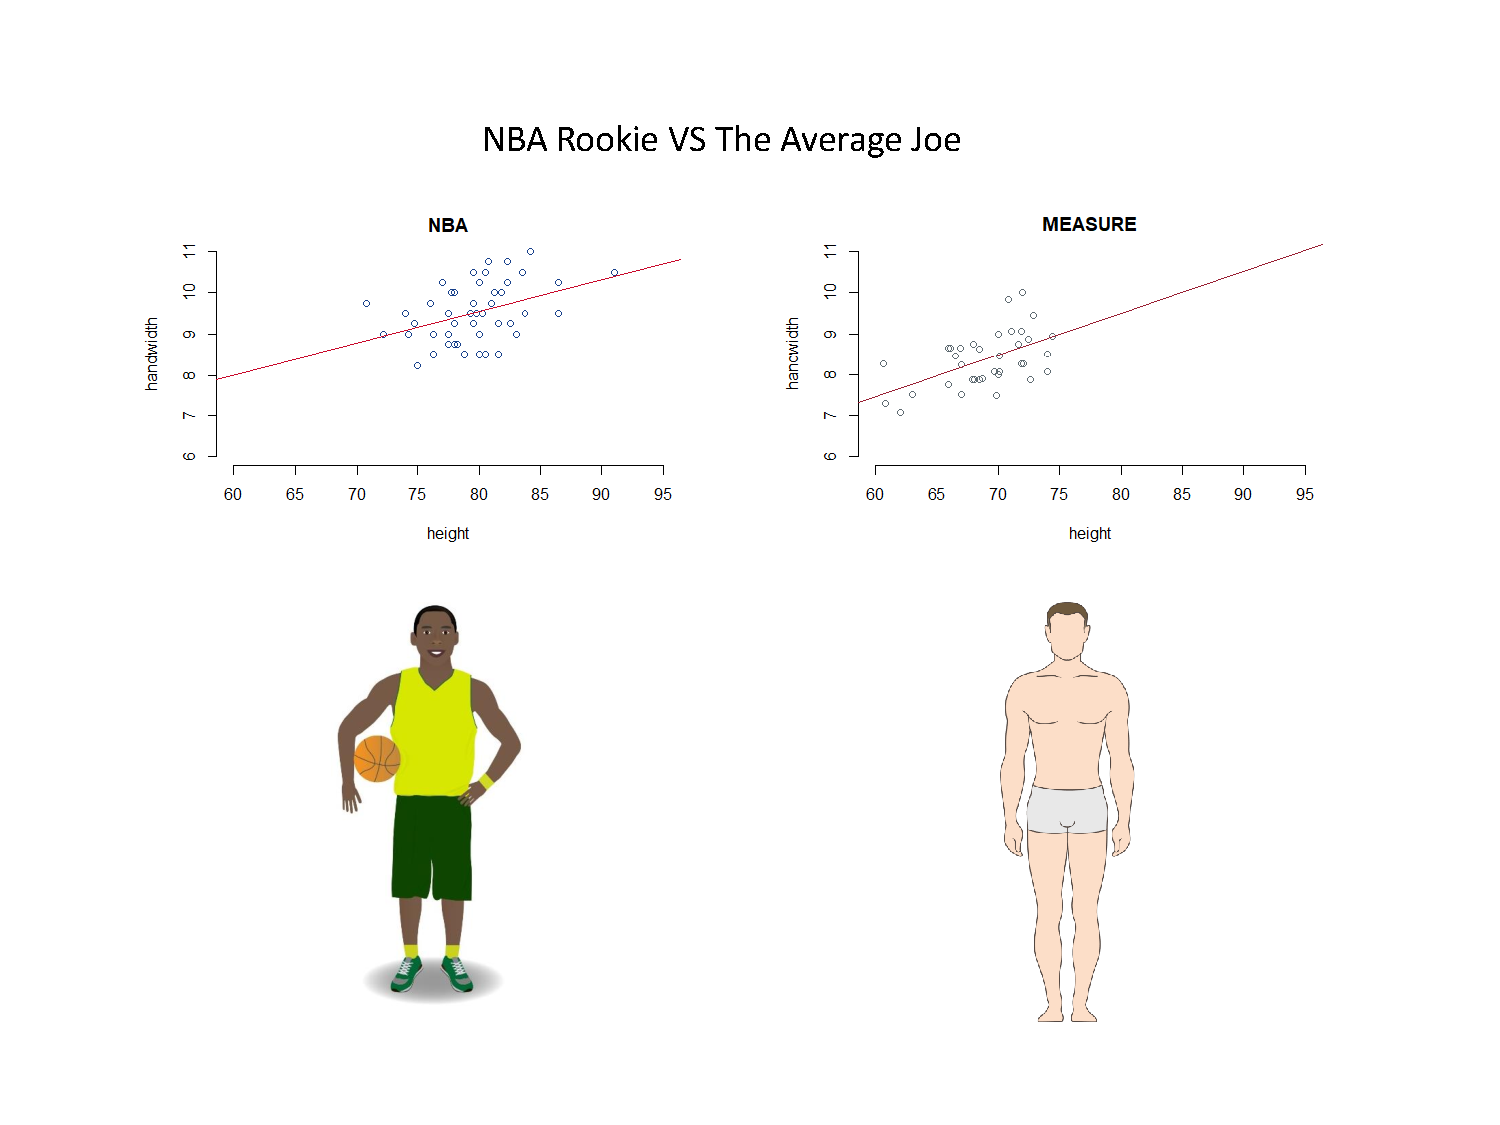
\includegraphics[trim = 0 0 0 0,clip,width=0.85\textwidth]{pdfs/oneimage.pdf} }
    \end{center}
    \label{fig:oneimage-1}
    \caption{ \textbf{One Image Description:} On the left represents a NBA rookies hand width vs height proportions of hand. On the right you can see your average Joe (the student volunteers measured).}
    \hrule
\end{figure}

\newpage

\section{Research Question:  What is my primary question}
\label{sec:rq}

How do NBA rookies differ from student volunteers?

\subsection{What is my secondary question}
\label{sec:rq2}

My secondary question is to see if NBA rookies hand width proportion to
height extremely differs when looking and hand width proportions to
height for the measurement on students volunteers?

\subsection{What is my other secondary question}
\label{sec:rq3}

My other secondary question is to see what measurements have the
strongest correlation with our measured volunteers when it comes to hand
width, with other body parts?

\section{Data Description}
\label{sec:data}

The collection of my data was done via a handout I made found
\ref{fig:handout-1} and \ref{fig:handout-2} in
section\textasciitilde{}\ref{sec:appendix-data-handout}. This handout
took various measurements and questions regarding things like height,
weight, length, dominant hand, etc. I went about collecting this data
via email. My data was targeted towards family and closed friends. This
data was targeted toward family and friend as there is a
pandemic\ldots{} The data was collected for the purpoase of this
project. I then merged with the rest of my class data that consist of
other students measures that they preformed on volunteers. This combined
gave the class a data set of 463 volunteers. \newline

\noindent When searching for data I went to Google and found the NBA
website, refer to the references where I cited \citet{NBAdata}. There I
found useful data that related to my measurements I took. The data
consisted of NBA rookies hand width, hand length, height, standing
reach, wingspan, weight, body fat, and position. The data I used was
specifically for 2019 NBA rookies.

\subsection{Summary of Sample}
\label{sec:data-sample}

The measure volunteer data was narrowed down to only people who are Male
as there are no females in the NBA. I also filtered about those who are
not between the ages of 18-28. I chose that age range as I think that is
the most relevant age for a rookie. I then went on the filter out those
who's standing reach was shorter then their height. Lastly, I selected
random males from both data sets to do observations on.

\subsection{Summary Statistics of Data}
\label{sec:data-summary}

Once my data was cleaned, I then selected the relevant data columns to
use for my observations. Those being player/volunteer, hand width, hand
length, standing reach, wingspan, and height. Those variables were
selected for both data sets. The analysis that was done on the selected
data sets consisted of correlations, boxplots, hierarchical clustering,
and t tests.

\newpage

\begin{table}[!htbp]
\footnotesize
\centering
\caption{\textbf{Descriptive Statistics and Correlation Analysis (NBA)}}
\label{table:correlation-nba}
\begin{tabularx}{0.9\textwidth}{{r@{ \ \ } p{35mm} r@{}lp{1mm} r@{}l p{5mm} r@{}l p{2mm} r@{}l p{2mm} r@{}l p{2mm} r@{}l p{2mm}   r@{}l  }}
 & \\
\hline
 & \\
\multicolumn{2}{c}{\textbf{ }} & \multicolumn{2}{c}{\textbf{M}} & & \multicolumn{2}{c}{\textbf{SD}} &  & \multicolumn{2}{c}{\textbf{1}} &  & \multicolumn{2}{c}{\textbf{2}} &  & \multicolumn{2}{c}{\textbf{3}} &  & \multicolumn{2}{c}{\textbf{4}} &  & \\ 
 & \\
\hline
 & \\
\textbf{1} & \textbf{height} &  79&.2 &  &  3&.78 &  &  1&  &  &  \multicolumn{2}{c}{ \  \  \  \  \ }  &  &  \multicolumn{2}{c}{ \  \  \  \  \ }  &  &  \multicolumn{2}{c}{ \  \  \  \  \ }  &  & \\ 
 & \\
\textbf{2} & \textbf{wingspan} &  82&.6 &  &  4&.49 &  &  &.90{$^{***}$}  &  &  1&  &  &  \multicolumn{2}{c}{ \  \  \  \  \ }  &  &  \multicolumn{2}{c}{ \  \  \  \  \ }  &  & \\ 
 & \\
\textbf{3} & \textbf{standing.reach} &  103&.7 &  &  5&.59 &  &  &.96{$^{***}$}  &  &  &.95{$^{***}$}  &  &  1&  &  &  \multicolumn{2}{c}{ \  \  \  \  \ }  &  & \\ 
 & \\
\textbf{4} & \textbf{hand.length} &  8&.8 &  &  &.60 &  &  &.75{$^{***}$}  &  &  &.88{$^{***}$}  &  &  &.84{$^{***}$}  &  &  1&  &  & \\ 
 & \\
\textbf{5} & \textbf{hand.width} &  9&.5 &  &  &.71 &  &  &.47{$^{***}$}  &  &  &.52{$^{***}$}  &  &  &.51{$^{***}$}  &  &  &.65{$^{***}$}  &  & \\ 
 & \\
\hline
 & \\
\multicolumn{19}{p{0.81\textwidth}}{  \footnotesize { \begin{hangparas}{0.75in}{1} \textbf{\underline{Notes}:} \ \ Pearson pairwise correlations are reported; \newline a two-side test was performed to report correlation significance.  \end{hangparas} } }  & \\  
\multicolumn{19}{p{0.81\textwidth}}{  {\tiny {$^{\dagger} p < .10$} }  {     } {\tiny        {$^{*} p < .05$} }  {     } {\tiny       {$^{**} p < .01$} }  {     } {\tiny      {$^{***} p < .001$} } {     }     } & \\ 
 & \\
\hline
\end{tabularx}
\end{table}
             
\begin{table}[!htbp]
\footnotesize
\centering
\caption{\textbf{Descriptive Statistics and Correlation Analysis (MEASURE)}}
\label{table:correlation-student-measure}
\begin{tabularx}{0.9\textwidth}{{r@{ \ \ } p{35mm} r@{}lp{1mm} r@{}l p{5mm} r@{}l p{2mm} r@{}l p{2mm} r@{}l p{2mm} r@{}l p{2mm}   r@{}l  }}
 & \\
\hline
 & \\
\multicolumn{2}{c}{\textbf{ }} & \multicolumn{2}{c}{\textbf{M}} & & \multicolumn{2}{c}{\textbf{SD}} &  & \multicolumn{2}{c}{\textbf{1}} &  & \multicolumn{2}{c}{\textbf{2}} &  & \multicolumn{2}{c}{\textbf{3}} &  & \multicolumn{2}{c}{\textbf{4}} &  & \\ 
 & \\
\hline
 & \\
\textbf{1} & \textbf{height} &  69&.4 &  &  3&.72 &  &  1&  &  &  \multicolumn{2}{c}{ \  \  \  \  \ }  &  &  \multicolumn{2}{c}{ \  \  \  \  \ }  &  &  \multicolumn{2}{c}{ \  \  \  \  \ }  &  & \\ 
 & \\
\textbf{2} & \textbf{wingspan} &  69&.8 &  &  4&.09 &  &  &.79{$^{***}$}  &  &  1&  &  &  \multicolumn{2}{c}{ \  \  \  \  \ }  &  &  \multicolumn{2}{c}{ \  \  \  \  \ }  &  & \\ 
 & \\
\textbf{3} & \textbf{standing.reach} &  86&.7 &  &  5&.32 &  &  &.88{$^{***}$}  &  &  &.83{$^{***}$}  &  &  1&  &  &  \multicolumn{2}{c}{ \  \  \  \  \ }  &  & \\ 
 & \\
\textbf{4} & \textbf{hand.length} &  7&.6 &  &  &.43 &  &  &.55{$^{***}$}  &  &  &.45{$^{**}$}  &  &  &.31{$^{\dagger}$}  &  &  1&  &  & \\ 
 & \\
\textbf{5} & \textbf{hand.width} &  8&.4 &  &  &.67 &  &  &.53{$^{***}$}  &  &  &.57{$^{***}$}  &  &  &.48{$^{**}$}  &  &  &.56{$^{***}$}  &  & \\ 
 & \\
\hline
 & \\
\multicolumn{19}{p{0.81\textwidth}}{  \footnotesize { \begin{hangparas}{0.75in}{1} \textbf{\underline{Notes}:} \ \ Pearson pairwise correlations are reported; \newline a two-side test was performed to report correlation significance.  \end{hangparas} } }  & \\  
\multicolumn{19}{p{0.81\textwidth}}{  {\tiny {$^{\dagger} p < .10$} }  {     } {\tiny        {$^{*} p < .05$} }  {     } {\tiny       {$^{**} p < .01$} }  {     } {\tiny      {$^{***} p < .001$} } {     }     } & \\ 
 & \\
\hline
\end{tabularx}
\end{table}


\subsection{Summary of Correlation}
\label{sec:correlation}

When looking at the correlation of NBA rookies measurements, the
standing arm reach and height have the highest correlation at 96\%. But
there are many other high correlated variables such as wingspan and
standing reach with a 95\% correlation and the wingspan and height with
a 90\% correlation. \newline

\noindent When looking at the measure of students volunteers there seems
to be the strongest correlation between standing arm reach and height at
88\%. Secondly, standing reach and wingspan have a high correlation at
83\%. Looking at what measurements correlate the least it would be
students height and hand width with a 53\% correlation. \newline

\noindent I then preformed a t test for NBA hand width and students hand
width to get a p value \textless{} .05 so I rejected the null hypothesis
that they are similar and conclude that nba rookies have larger hands. I
went on to preform t test for NBA and volunteers height, wingspan, and
standing reach to find all p values \textless{} .05.

\section{Key Findings}
\label{sec:findings}

Proportionally NBA rookies have smaller height in hand proportions, this
is because they have larger hands therefore smaller height proportions
then students when compared to hand size. You can also see that NBA
rookies are bigger larger in general. You can see that by observing the
t test, plots, and correlations charts in the appendices. \newline

\noindent I also found it interesting that for our measure volunteers
the correlation between hand length and height was only 45\% but with
NBA rookies it was much higher at 88\%. This leads me to believe that
there was some fabricated or bad data recorded from some of the
students.

\section{Conclusion}
\label{sec:conclusion}

When looking at the volunteers for the measure data I found that the
highest correlated variables were standing reach and height. The highest
correlated variables for the NBA rookies were also standing reach and
height. When comparing NBA hand size proportions you can see the NBA
rookies have a lower height proportion than the measure volunteers. Thus
meaning NBA rookies have large hands compared to measure volunteers.
Lastly, NBA rookies have larger means implying they're overall just
bigger people. \newline

\noindent I concluded that the NBA has a precise and very accurate way
for measuring rookies and the measurements taken by students may very.
That is due to some students not understanding how to take the correct
measure. But it also appears some students have fabricated their data.
It is also suspicious when one of the volunteers was only about 6 feet
tall, yet has a 8 foot wing span\ldots{} Therefore, a re evaluation of
this analysis with more accurate measurements may differ the results.

\section{APPENDICES}
\label{sec:appendix}

\subsection{Data Provenance}
\label{sec:appendix-data-provenance}

I made my handout and sent it out to 10 people to get the specific
measurements shown in the handout in figure \ref{fig:handout-1} and
\ref{fig:handout-2} in
section\textasciitilde{}\ref{sec:appendix-data-handout}. Those
measurement were taken in centimeters for a more precise measurement and
later converted to inches. I then made their data anonymous with a bitly
generator. After that I merged my data with classmates data to have a
larger data set. I then went on to randomly select 50 males to correlate
and compare my NBA rookie data from \citep{NBAdata} as there are not
women who play in the NBA. I started by merging columns, some columns
had only one hand measured so I took the left and rights averaging them
to create and single column. If there was only one measurement like only
left hand length, that would be selected. Out of all the measurements I
decided to look into the hand width, hand length, height, wingspan, and
standing reach. In that data there were all different ages so I narrowed
my ages down to 18-28 as those are the more likely ages to be a rookie
in the NBA. I found some people miss entered or miss measured their
data, in one case it was the arm reach. When standing some would measure
from shoulder to finger tip whereas that measurement should be from the
ground to finger tip. With that I filtered out those who measured the
standing reach to be shorter than the height. \newline

\noindent When looking deeper into the data I found some more anomalies
that caused my data to be skewed. My professor found corrupt data where
some students had entered some bad data and/or the data was fabricated.
With that our professor helped through the cleanup process narrowing
down from about 463 to 251 people from there I was able to re apply all
of my changes such as age restrictions, investigating of only males,
removed unused columns, etc. I finally ended up with 42 student
volunteers to compare with my NBA rookies. The clean up process and
approach my professor took can be found in references where I cite
\citep{MonteShaffer}. \newline

\noindent Once I was finished cleaning my NBA data I chose to look into
hand width, hand length, height, wingspan, and standing arms reach. For
this data I had to convert from feet and inches to just inches. I then
decided to look into if NBA rookies and our volunteers are abnormally
proportional to other parts of their body such as hand width relative to
their height. I chose to take proportions of hand width as I think
larger hands give a leverage in basketball so it would be interesting to
see how large these proportions are compared to the average person. I
found that on average NBA rookies are one whole hand size larger. That
meaning that they are either just bigger people in general or have
abnormally large hands. The means of each show you can see that
proportionally they are just larger people. Looking at
section\textasciitilde{}\ref{sec:hclust} you can also see that and that
similar groups are grouped together and it is the same for our
volunteers as . \newline

\noindent Moving forward if I were to re create this project I would
make precise measurements were taken. I would do so by having all
measurement taken in centimeters and all the same exact way. As I have
stated the NBA goes about a very detailed way of measuring rookies.
Moving forward another change I would make is to get more NBA data and
include the position. If I had position then I could specifically look
into what positions related more to each other, as well as potentially
make a classifier to predict what position a student is most likely to
play.

\begin{figure}[!ht]
    \hrule
    \begin{center}
        \scalebox{1.00}{    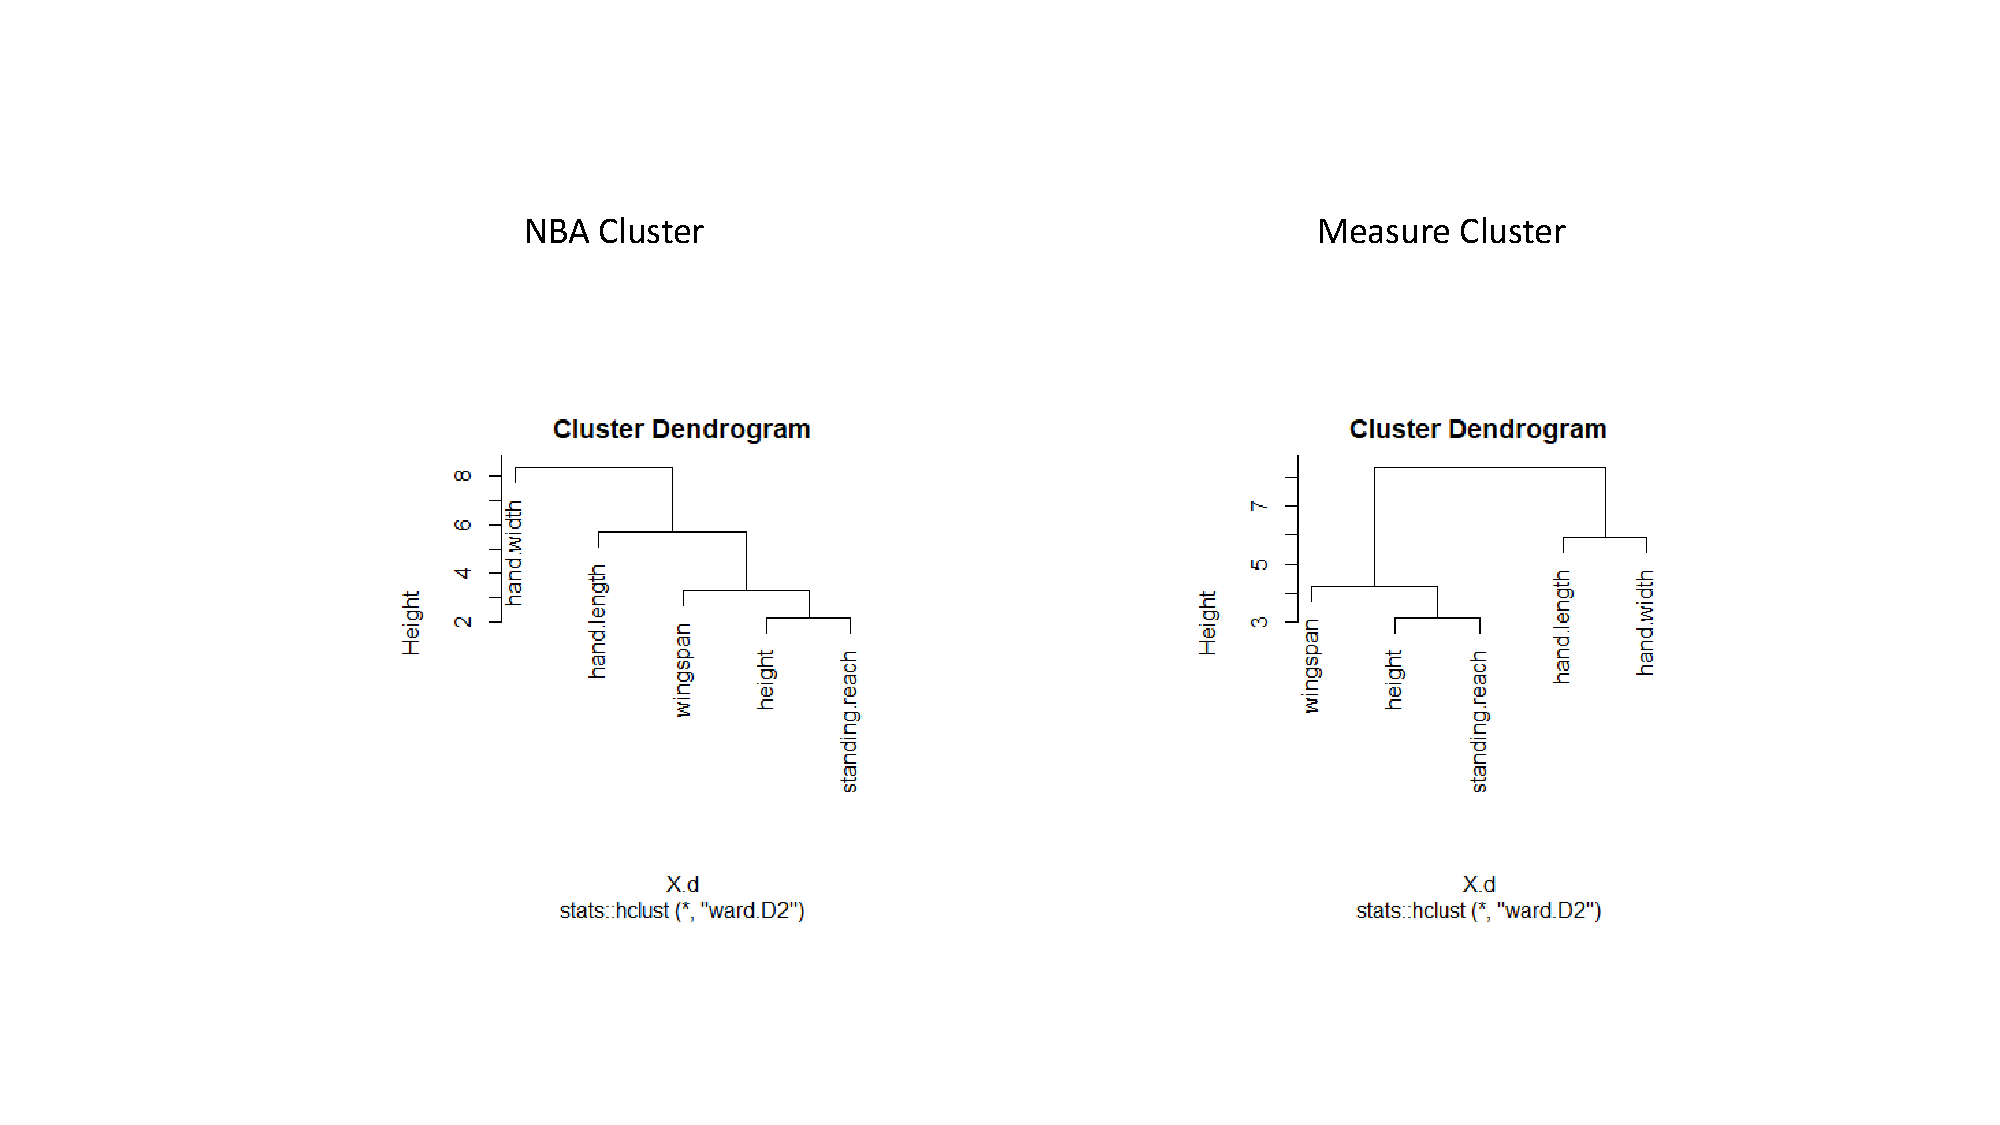
\includegraphics[trim = 0 0 0 0,clip,width=0.85\textwidth]{pdfs/handout3.pdf} }
    \end{center}
    \label{fig:handout-3}
    \caption{ \textbf{Cluster of like measurements:} On the left is a cluster of NBA measurements and on the right is a cluster of student volunteers measurements}
    \hrule
\end{figure}

\newpage

\subsubsection{Data Collection Handout}
\label{sec:appendix-data-handout}

\begin{figure}[!ht]
    \hrule
    \caption{ \textbf{Handout Page 1} }
    \begin{center}
        \scalebox{1.00}{    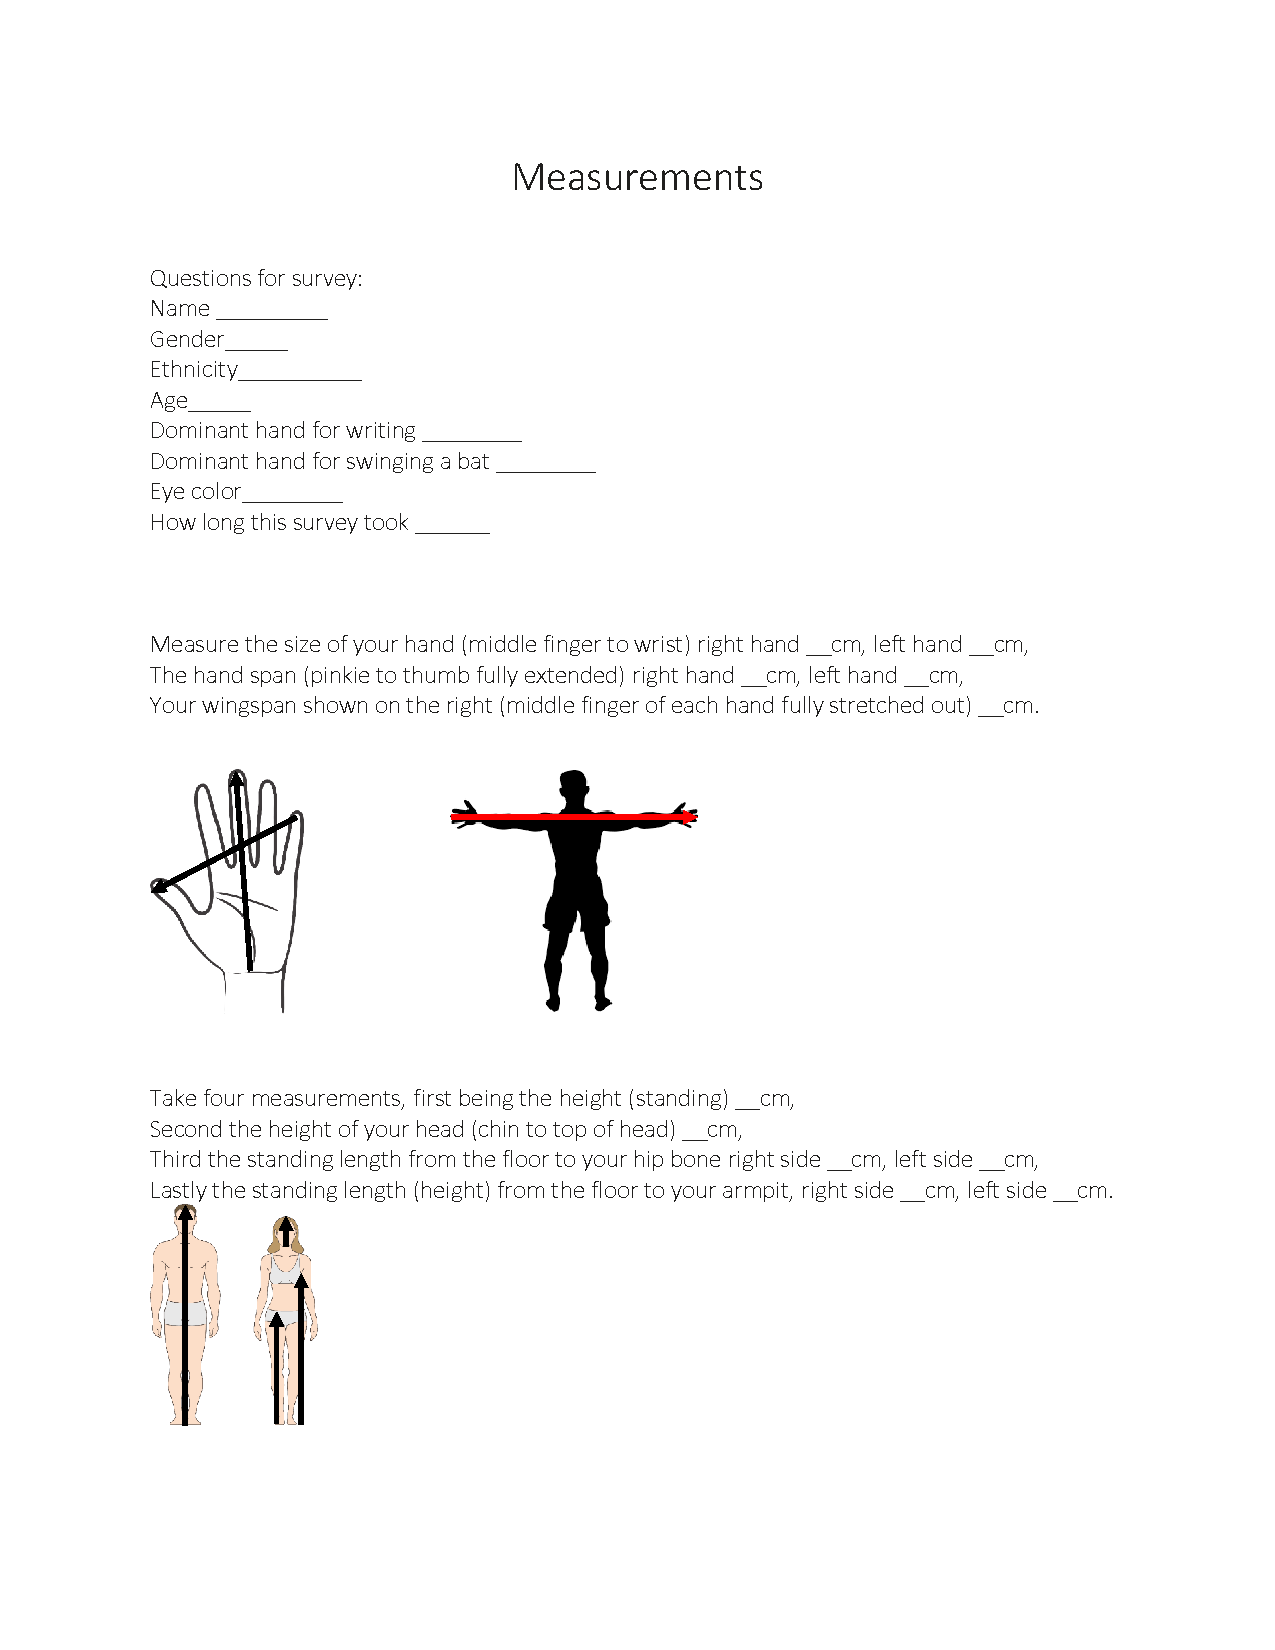
\includegraphics[trim = 0 0 0 0,clip,width=0.85\textwidth]{pdfs/handout1.pdf} }
    \end{center}
    \label{fig:handout-1}
    \hrule
\end{figure}

\newpage

\begin{figure}[!ht]
    \hrule
    \caption{ \textbf{Handout Page 2} }
    \begin{center}
        \scalebox{1.00}{    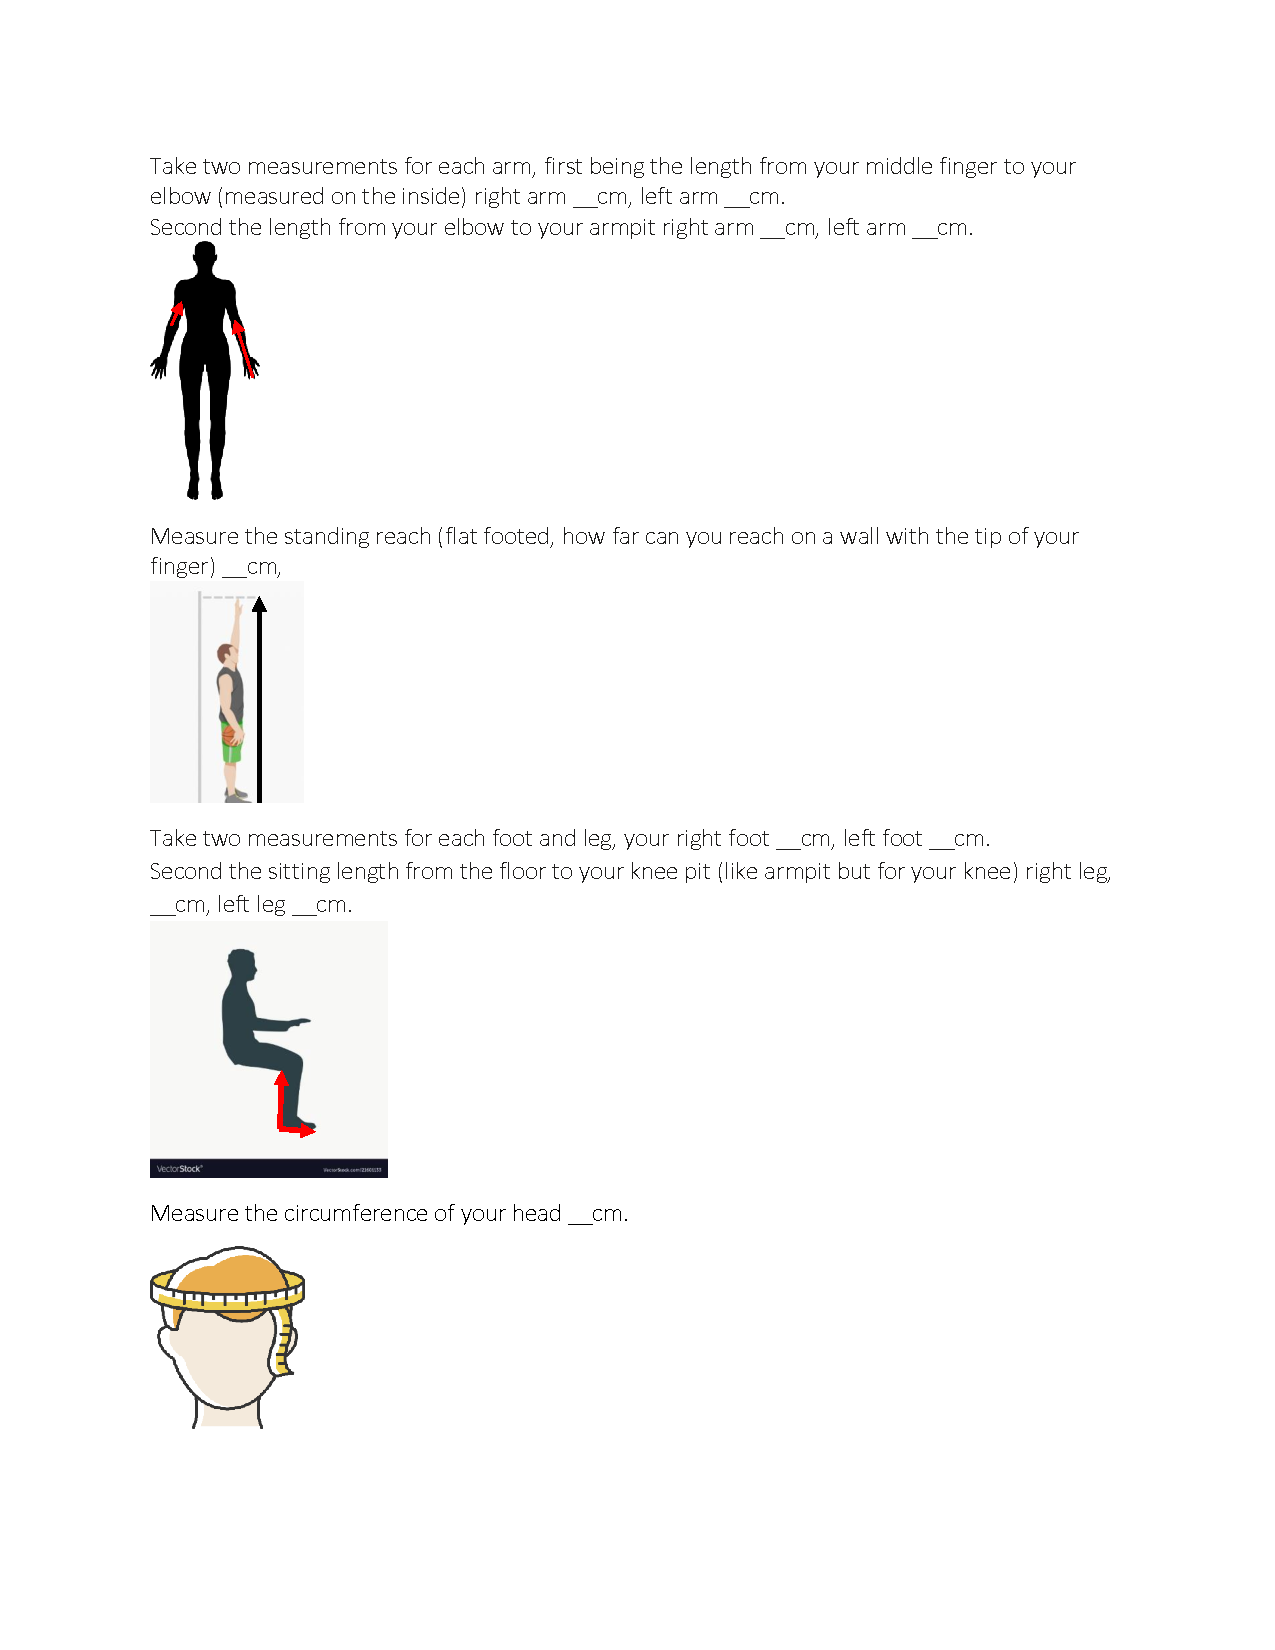
\includegraphics[trim = 0 0 0 0,clip,width=0.85\textwidth]{pdfs/handout2.pdf} }
    \end{center}
    \label{fig:handout-2}
    \hrule
\end{figure}

\newpage

\subsection{Preparing the Report}
\label{sec:necessary-functions}

Below is the necessary functions and libraries required to run the code
referenced in this document.

\begin{Shaded}
\begin{Highlighting}[]
\KeywordTok{library}\NormalTok{(devtools);       }\CommentTok{\# required for source\_url}
\end{Highlighting}
\end{Shaded}

\begin{verbatim}
## Warning: package 'devtools' was built under R version 4.0.3
\end{verbatim}

\begin{Shaded}
\begin{Highlighting}[]
\KeywordTok{library}\NormalTok{(humanVerseWSU)}

\NormalTok{path.humanVerseWSU =}\StringTok{ "https://raw.githubusercontent.com/MonteShaffer/humanVerseWSU/"}
\KeywordTok{source\_url}\NormalTok{( }\KeywordTok{paste0}\NormalTok{(path.humanVerseWSU,}\StringTok{"master/misc/functions{-}project{-}measure.R"}\NormalTok{) );}
\end{Highlighting}
\end{Shaded}

\begin{verbatim}
## Warning: package 'survival' was built under R version 4.0.3
\end{verbatim}

\begin{verbatim}
## Warning: package 'Formula' was built under R version 4.0.3
\end{verbatim}

\begin{Shaded}
\begin{Highlighting}[]
\NormalTok{path.github =}\StringTok{ "https://raw.githubusercontent.com/njtrout/WSU\_STATS419\_FALL2020/"}
\KeywordTok{source\_url}\NormalTok{( }\KeywordTok{paste0}\NormalTok{(path.github,}\StringTok{"master/functions/functions{-}project{-}measure.R"}\NormalTok{) );}

\NormalTok{path.project =}\StringTok{ "C:/Users/Nic Trout/Documents/C/WSU\_STATS419\_FALL2020/project{-}measure\_nic/"}\NormalTok{;}
\NormalTok{path.to.secret =}\StringTok{ "C:/Users/Nic Trout/Desktop/"}\NormalTok{;}
\NormalTok{measure =}\StringTok{ }\KeywordTok{readRDS}\NormalTok{(}\KeywordTok{paste0}\NormalTok{(path.to.secret, }\StringTok{"final.measure.rds"}\NormalTok{));}
\NormalTok{nbadata =}\StringTok{ }\KeywordTok{read.csv}\NormalTok{(}\StringTok{"C:/Users/Nic Trout/Documents/C/WSU\_STATS419\_FALL2020/project{-}measure\_nic/nbadata.txt"}\NormalTok{, }\DataTypeTok{sep =}\StringTok{"}\CharTok{\textbackslash{}t}\StringTok{"}\NormalTok{, }\DataTypeTok{header =} \OtherTok{TRUE}\NormalTok{);}

\NormalTok{nba.df =}\StringTok{ }\KeywordTok{prepareDataNBA}\NormalTok{(nbadata);}
\end{Highlighting}
\end{Shaded}

\begin{verbatim}
## Warning in prepareDataNBA(nbadata): NAs introduced by coercion
\end{verbatim}

\begin{verbatim}
## Warning in prepareDataNBA(nbadata): NAs introduced by coercion
\end{verbatim}

\begin{Shaded}
\begin{Highlighting}[]
\NormalTok{measure.df =}\StringTok{ }\KeywordTok{prepareMeasureData}\NormalTok{(measure);}
\NormalTok{proportions =}\StringTok{ }\KeywordTok{getProportionHandWidthMeasure}\NormalTok{(measure.df);}
\NormalTok{proportionsNBA =}\StringTok{ }\KeywordTok{getProportionHandWidthNBA}\NormalTok{(nba.df);}
\end{Highlighting}
\end{Shaded}

\subsubsection{Plots}
\label{sec:plots}

\begin{Shaded}
\begin{Highlighting}[]
\CommentTok{\#height vs standing reach}
\KeywordTok{plotcorrS}\NormalTok{(           }\DataTypeTok{x.m =}\NormalTok{ measure.df}\OperatorTok{$}\NormalTok{height,}
                     \DataTypeTok{y.m =}\NormalTok{ measure.df}\OperatorTok{$}\NormalTok{standing.reach,}
                     \DataTypeTok{x.n =}\NormalTok{ nba.df}\OperatorTok{$}\NormalTok{height,}
                     \DataTypeTok{y.n =}\NormalTok{ nba.df}\OperatorTok{$}\NormalTok{standing.reach,}
                     \DataTypeTok{xl =} \StringTok{"height(inches)"}\NormalTok{,}
                     \DataTypeTok{yl =} \StringTok{"standing.reach(inches)"}\NormalTok{)}
\end{Highlighting}
\end{Shaded}

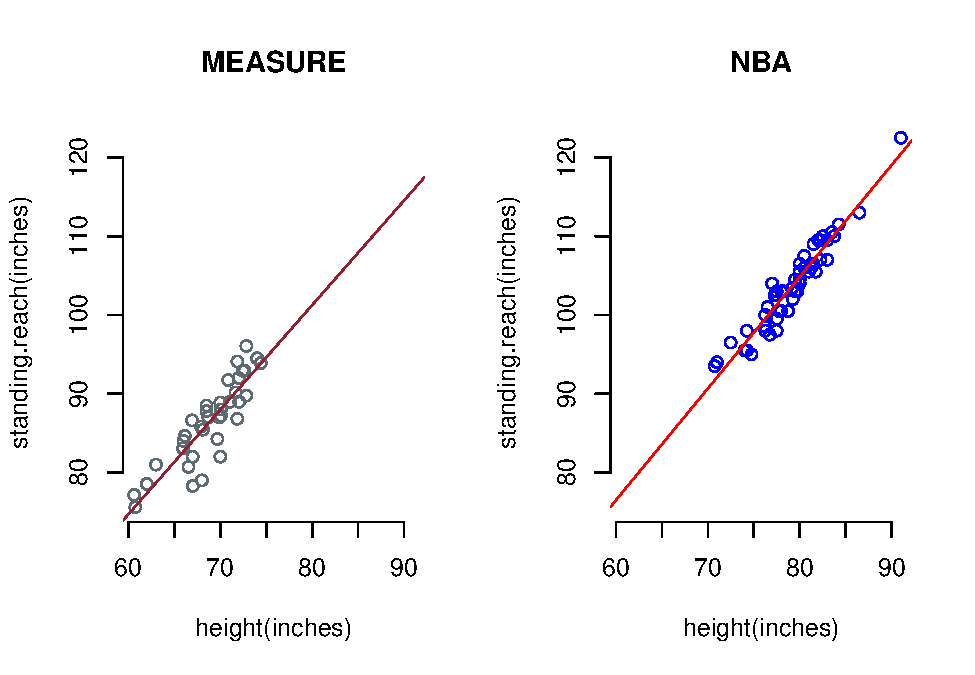
\includegraphics{project-measure-writeup_files/figure-latex/plots-and-ttest-1.pdf}

\begin{verbatim}
##       x.n 
## 0.6707615
\end{verbatim}

\begin{Shaded}
\begin{Highlighting}[]
\CommentTok{\#height{-}vs{-}hand width}
\KeywordTok{plotcorrS}\NormalTok{(           }\DataTypeTok{x.m =}\NormalTok{ measure.df}\OperatorTok{$}\NormalTok{height,}
                     \DataTypeTok{y.m =}\NormalTok{ measure.df}\OperatorTok{$}\NormalTok{hand.width,}
                     \DataTypeTok{x.n =}\NormalTok{ nba.df}\OperatorTok{$}\NormalTok{height,}
                     \DataTypeTok{y.n =}\NormalTok{ nba.df}\OperatorTok{$}\NormalTok{hand.width,}
                     \DataTypeTok{xl =} \StringTok{"height(inches)"}\NormalTok{,}
                     \DataTypeTok{yl =} \StringTok{"hand.width(inches)"}\NormalTok{)}
\end{Highlighting}
\end{Shaded}

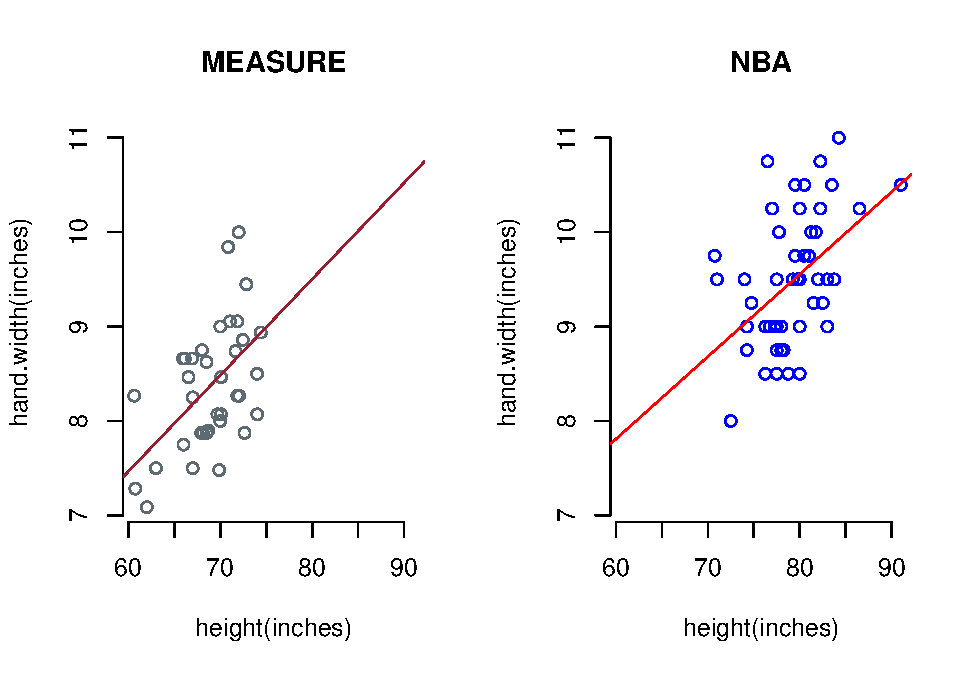
\includegraphics{project-measure-writeup_files/figure-latex/plots-and-ttest-2.pdf}

\begin{verbatim}
##        x.n 
## -0.4045789
\end{verbatim}

\begin{Shaded}
\begin{Highlighting}[]
\CommentTok{\#height{-}vs{-}wingspan}
\KeywordTok{plotcorrS}\NormalTok{(       }\DataTypeTok{x.m =}\NormalTok{ measure.df}\OperatorTok{$}\NormalTok{height,}
                     \DataTypeTok{y.m =}\NormalTok{ measure.df}\OperatorTok{$}\NormalTok{wingspan,}
                     \DataTypeTok{x.n =}\NormalTok{ nba.df}\OperatorTok{$}\NormalTok{height,}
                     \DataTypeTok{y.n =}\NormalTok{ nba.df}\OperatorTok{$}\NormalTok{wingspan,}
                     \DataTypeTok{xl =} \StringTok{"height(inches)"}\NormalTok{,}
                     \DataTypeTok{yl =} \StringTok{"wingspan(inches)"}\NormalTok{)}
\end{Highlighting}
\end{Shaded}

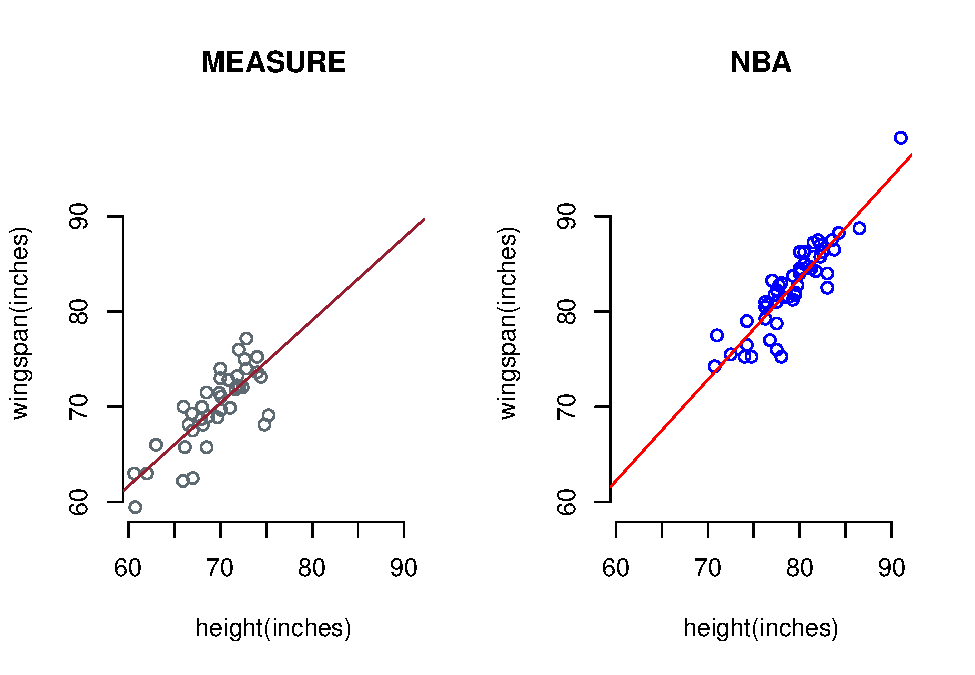
\includegraphics{project-measure-writeup_files/figure-latex/plots-and-ttest-3.pdf}

\begin{verbatim}
##      x.n 
## 1.426594
\end{verbatim}

\begin{Shaded}
\begin{Highlighting}[]
\CommentTok{\#nba/measure proportions, height to arm reach}
\KeywordTok{plotcorrS}\NormalTok{(           }\DataTypeTok{x.m =}\NormalTok{ proportions}\OperatorTok{$}\NormalTok{measure.height.proportion,}
                     \DataTypeTok{y.m =}\NormalTok{ proportions}\OperatorTok{$}\NormalTok{measure.armreach.proportion,}
                     \DataTypeTok{x.n =}\NormalTok{ proportionsNBA}\OperatorTok{$}\NormalTok{nba.df.height.proportion,}
                     \DataTypeTok{y.n =}\NormalTok{ proportionsNBA}\OperatorTok{$}\NormalTok{nba.df.armreach.proportion,}
                     \DataTypeTok{xl =} \StringTok{"ProportionHeight"}\NormalTok{,}
                     \DataTypeTok{yl =} \StringTok{"ProportionWingspan"}\NormalTok{)}
\end{Highlighting}
\end{Shaded}

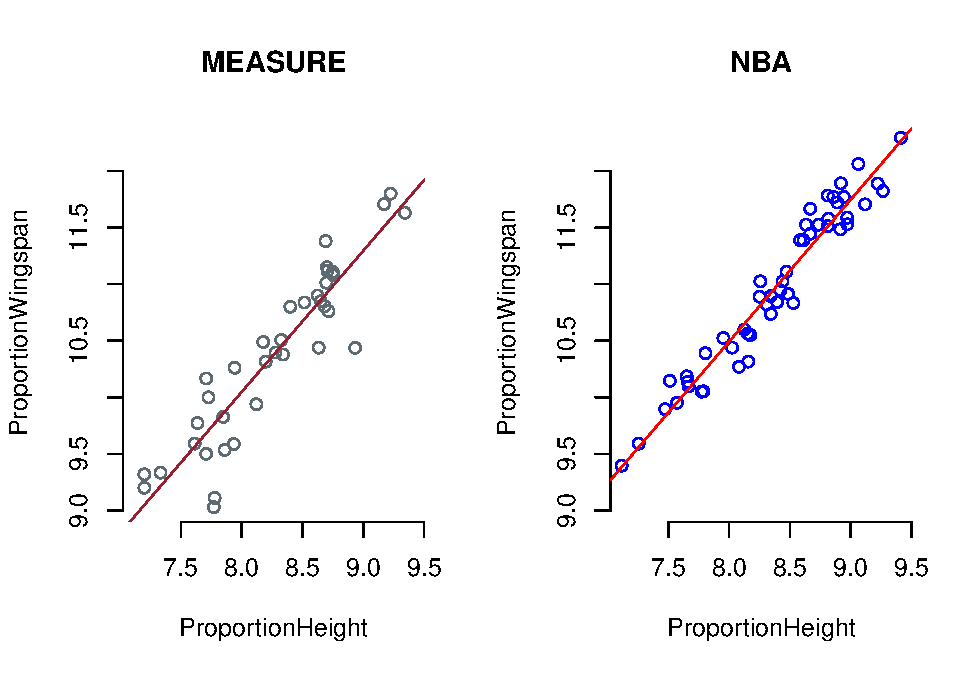
\includegraphics{project-measure-writeup_files/figure-latex/plots-and-ttest-4.pdf}

\begin{verbatim}
##        x.n 
## 0.06226467
\end{verbatim}

\subsubsection{T-tests}
\label{sec:Ttest}

\begin{Shaded}
\begin{Highlighting}[]
\KeywordTok{t.test}\NormalTok{(nba.df}\OperatorTok{$}\NormalTok{hand.width, measure.df}\OperatorTok{$}\NormalTok{hand.width, }\DataTypeTok{var.equal =} \OtherTok{FALSE}\NormalTok{)}
\end{Highlighting}
\end{Shaded}

\begin{verbatim}
## 
##  Welch Two Sample t-test
## 
## data:  nba.df$hand.width and measure.df$hand.width
## t = 7.3471, df = 81.5, p-value = 1.39e-10
## alternative hypothesis: true difference in means is not equal to 0
## 95 percent confidence interval:
##  0.7932888 1.3824488
## sample estimates:
## mean of x mean of y 
##  9.480000  8.392131
\end{verbatim}

\begin{Shaded}
\begin{Highlighting}[]
\KeywordTok{t.test}\NormalTok{(nba.df}\OperatorTok{$}\NormalTok{hand.length, measure.df}\OperatorTok{$}\NormalTok{hand.length, }\DataTypeTok{var.equal =} \OtherTok{FALSE}\NormalTok{)}
\end{Highlighting}
\end{Shaded}

\begin{verbatim}
## 
##  Welch Two Sample t-test
## 
## data:  nba.df$hand.length and measure.df$hand.length
## t = 10.622, df = 87.284, p-value < 2.2e-16
## alternative hypothesis: true difference in means is not equal to 0
## 95 percent confidence interval:
##  0.9367467 1.3680131
## sample estimates:
## mean of x mean of y 
##   8.77000   7.61762
\end{verbatim}

\begin{Shaded}
\begin{Highlighting}[]
\KeywordTok{t.test}\NormalTok{(nba.df}\OperatorTok{$}\NormalTok{height, measure.df}\OperatorTok{$}\NormalTok{height, }\DataTypeTok{var.equal =} \OtherTok{FALSE}\NormalTok{)}
\end{Highlighting}
\end{Shaded}

\begin{verbatim}
## 
##  Welch Two Sample t-test
## 
## data:  nba.df$height and measure.df$height
## t = 12.204, df = 82.341, p-value < 2.2e-16
## alternative hypothesis: true difference in means is not equal to 0
## 95 percent confidence interval:
##   8.179363 11.364879
## sample estimates:
## mean of x mean of y 
##  79.15500  69.38288
\end{verbatim}

\begin{Shaded}
\begin{Highlighting}[]
\KeywordTok{t.test}\NormalTok{(nba.df}\OperatorTok{$}\NormalTok{wingspan, measure.df}\OperatorTok{$}\NormalTok{wingspan, }\DataTypeTok{var.equal =} \OtherTok{FALSE}\NormalTok{)}
\end{Highlighting}
\end{Shaded}

\begin{verbatim}
## 
##  Welch Two Sample t-test
## 
## data:  nba.df$wingspan and measure.df$wingspan
## t = 14.154, df = 86.481, p-value < 2.2e-16
## alternative hypothesis: true difference in means is not equal to 0
## 95 percent confidence interval:
##  11.01493 14.61442
## sample estimates:
## mean of x mean of y 
##  82.58500  69.77032
\end{verbatim}

\begin{Shaded}
\begin{Highlighting}[]
\KeywordTok{t.test}\NormalTok{(proportionsNBA}\OperatorTok{$}\NormalTok{nba.df.height.proportion, proportions}\OperatorTok{$}\NormalTok{measure.height.proportion, }\DataTypeTok{var.equal =} \OtherTok{FALSE}\NormalTok{)}
\end{Highlighting}
\end{Shaded}

\begin{verbatim}
## 
##  Welch Two Sample t-test
## 
## data:  proportionsNBA$nba.df.height.proportion and proportions$measure.height.proportion
## t = 0.93993, df = 77.082, p-value = 0.3502
## alternative hypothesis: true difference in means is not equal to 0
## 95 percent confidence interval:
##  -0.1273886  0.3551791
## sample estimates:
## mean of x mean of y 
##  8.381208  8.267313
\end{verbatim}

\subsubsection{Boxplots}
\label{sec:boxplots}

\begin{Shaded}
\begin{Highlighting}[]
\KeywordTok{boxplotfunc}\NormalTok{(proportionsNBA}\OperatorTok{$}\NormalTok{nba.df.height.proportion, proportions}\OperatorTok{$}\NormalTok{measure.height.proportion, measure.df}\OperatorTok{$}\NormalTok{hand.width, nba.df}\OperatorTok{$}\NormalTok{hand.width);}
\end{Highlighting}
\end{Shaded}

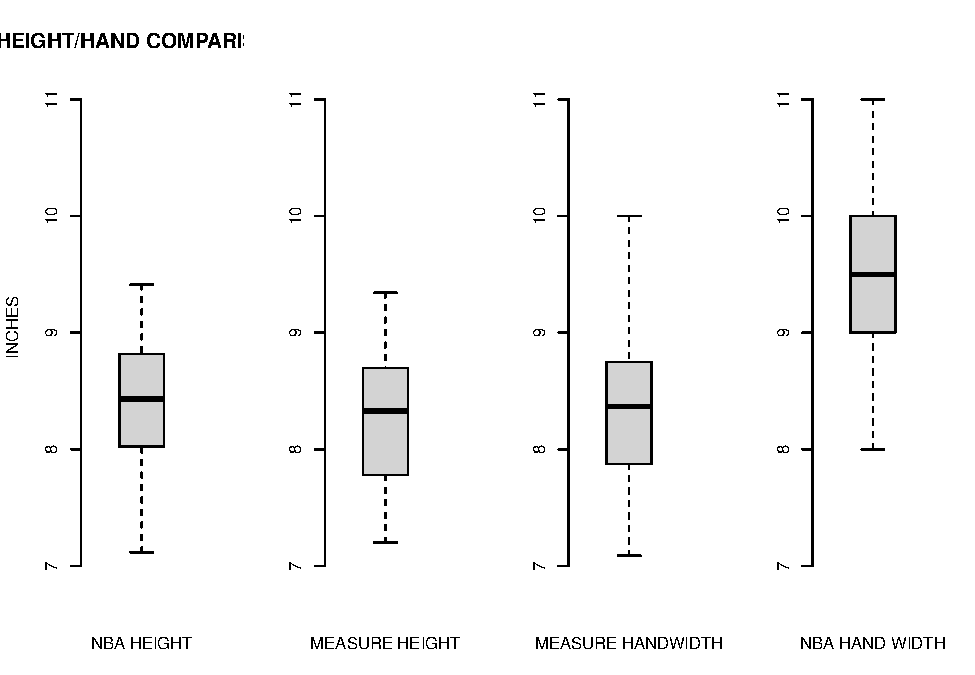
\includegraphics{project-measure-writeup_files/figure-latex/boxplots-hand/height-proportions-1.pdf}

\subsubsection{Hclust}
\label{sec:hclust}

\begin{Shaded}
\begin{Highlighting}[]
\KeywordTok{source\_url}\NormalTok{( }\KeywordTok{paste0}\NormalTok{(path.humanVerseWSU,}\StringTok{"master/humanVerseWSU/R/functions{-}EDA.R"}\NormalTok{) );}
\end{Highlighting}
\end{Shaded}

\begin{verbatim}
## SHA-1 hash of file is dd72e464241952b23d5b08d2213099eccf7a86f6
\end{verbatim}

\begin{verbatim}
## Welcome! Want to learn more? See two factoextra-related books at https://goo.gl/ve3WBa
\end{verbatim}

\begin{verbatim}
## 
## Attaching package: 'psych'
\end{verbatim}

\begin{verbatim}
## The following object is masked from 'package:Hmisc':
## 
##     describe
\end{verbatim}

\begin{verbatim}
## The following objects are masked from 'package:ggplot2':
## 
##     %+%, alpha
\end{verbatim}

\begin{Shaded}
\begin{Highlighting}[]
\NormalTok{Xs =}\StringTok{ }\KeywordTok{scale}\NormalTok{(nba.df[,}\KeywordTok{c}\NormalTok{(}\DecValTok{1}\NormalTok{,}\DecValTok{2}\NormalTok{,}\DecValTok{3}\NormalTok{,}\DecValTok{4}\NormalTok{,}\DecValTok{5}\NormalTok{)])}
\KeywordTok{rownames}\NormalTok{(Xs) =}\StringTok{ }\NormalTok{nba.df}\OperatorTok{$}\NormalTok{players           }
\NormalTok{do.nothing =}\StringTok{ }\KeywordTok{perform.hclust}\NormalTok{(Xs,}\DecValTok{12}\NormalTok{)}
\end{Highlighting}
\end{Shaded}

\begin{verbatim}
## Registered S3 method overwritten by 'dendextend':
##   method       from   
##   text.pvclust pvclust
\end{verbatim}

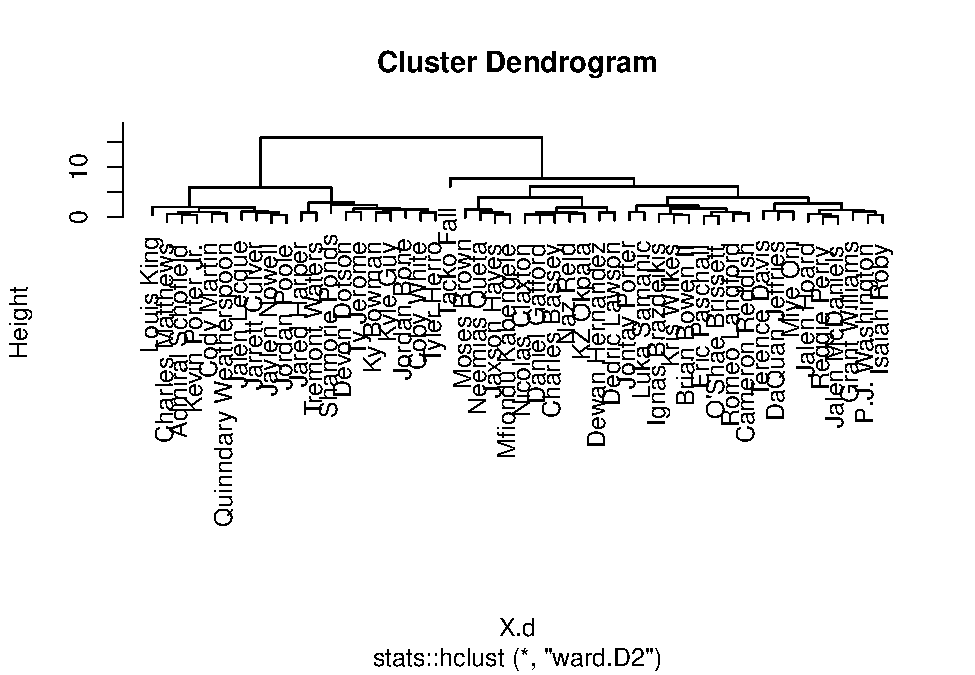
\includegraphics{project-measure-writeup_files/figure-latex/hclust-nbarookies-1.pdf}
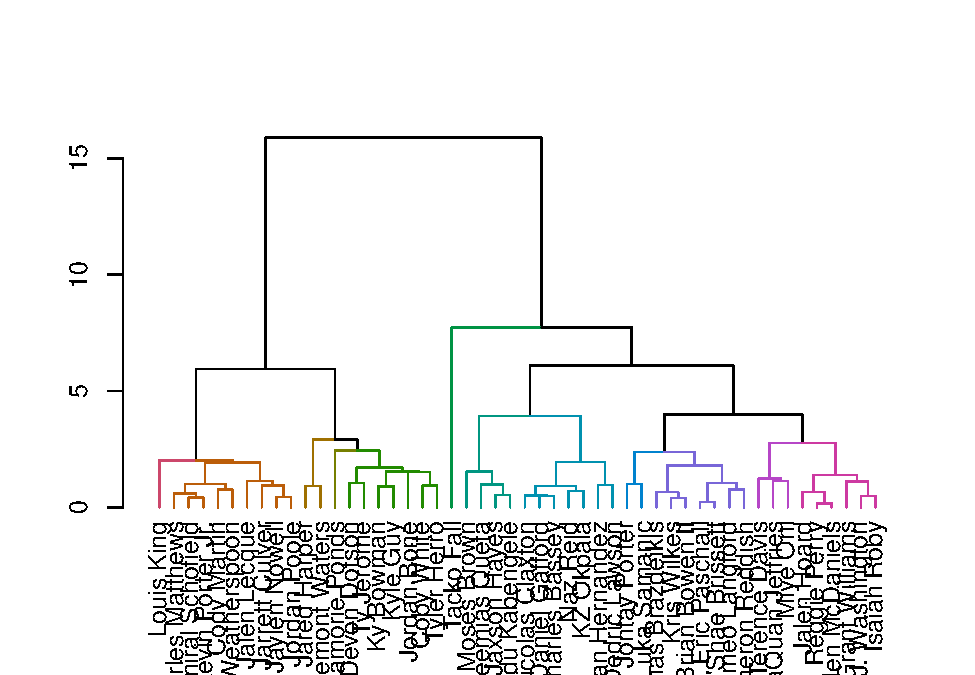
\includegraphics{project-measure-writeup_files/figure-latex/hclust-nbarookies-2.pdf}

\begin{verbatim}
## [1] "Pruning 1 of 12"
## [1] "Pruning 2 of 12"
## [1] "Pruning 3 of 12"
## [1] "Pruning 4 of 12"
## [1] "Pruning 5 of 12"
## [1] "Pruning 6 of 12"
## [1] "Pruning 7 of 12"
## [1] "Pruning 8 of 12"
## [1] "Pruning 9 of 12"
## [1] "Pruning 10 of 12"
## [1] "Pruning 11 of 12"
## [1] "Pruning 12 of 12"
\end{verbatim}

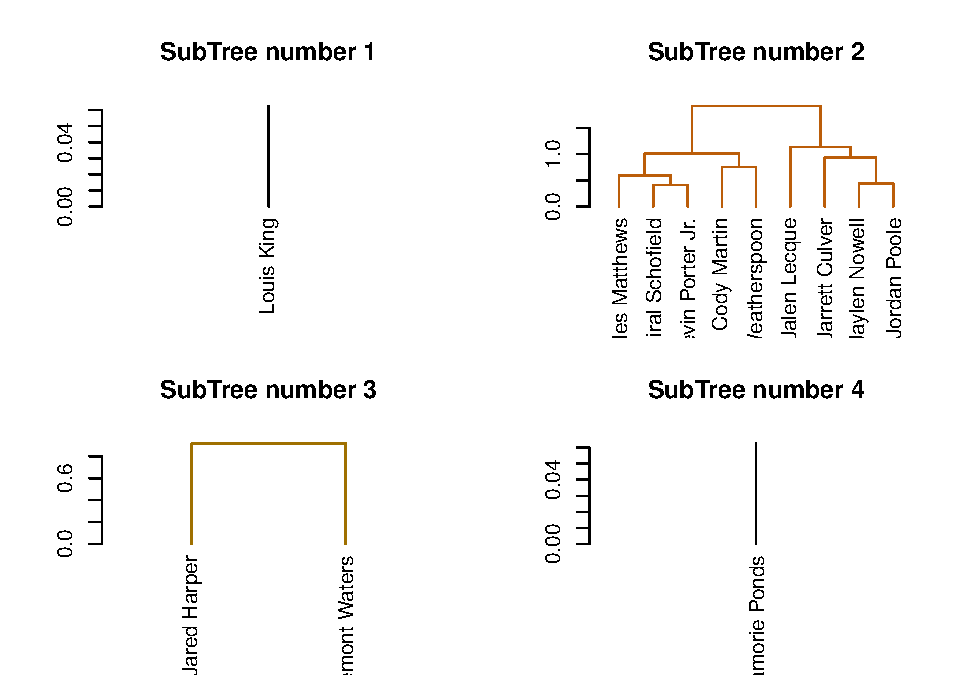
\includegraphics{project-measure-writeup_files/figure-latex/hclust-nbarookies-3.pdf}
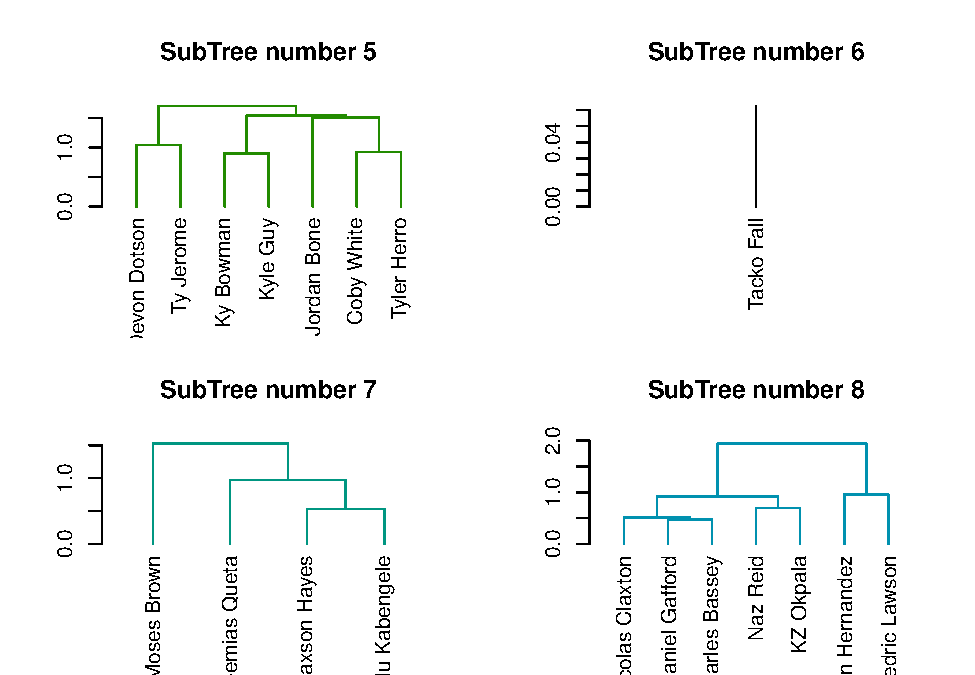
\includegraphics{project-measure-writeup_files/figure-latex/hclust-nbarookies-4.pdf}
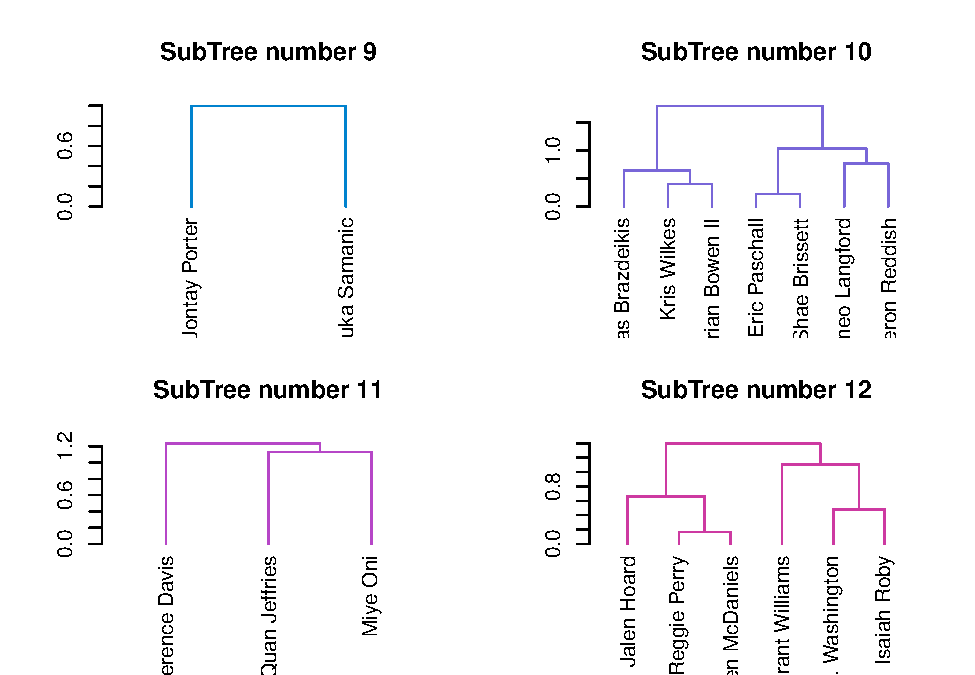
\includegraphics{project-measure-writeup_files/figure-latex/hclust-nbarookies-5.pdf}

\begin{Shaded}
\begin{Highlighting}[]
\KeywordTok{source\_url}\NormalTok{( }\KeywordTok{paste0}\NormalTok{(path.humanVerseWSU,}\StringTok{"master/humanVerseWSU/R/functions{-}EDA.R"}\NormalTok{) );}
\end{Highlighting}
\end{Shaded}

\begin{verbatim}
## SHA-1 hash of file is dd72e464241952b23d5b08d2213099eccf7a86f6
\end{verbatim}

\begin{Shaded}
\begin{Highlighting}[]
\NormalTok{Xs =}\StringTok{ }\KeywordTok{scale}\NormalTok{(nba.df[,}\KeywordTok{c}\NormalTok{(}\DecValTok{1}\NormalTok{,}\DecValTok{2}\NormalTok{,}\DecValTok{3}\NormalTok{,}\DecValTok{4}\NormalTok{,}\DecValTok{5}\NormalTok{)])}
\NormalTok{Xs =}\StringTok{ }\KeywordTok{transposeMatrix}\NormalTok{(Xs)}
\NormalTok{do.nothing =}\StringTok{ }\KeywordTok{perform.hclust}\NormalTok{(Xs,}\DecValTok{3}\NormalTok{)}
\end{Highlighting}
\end{Shaded}

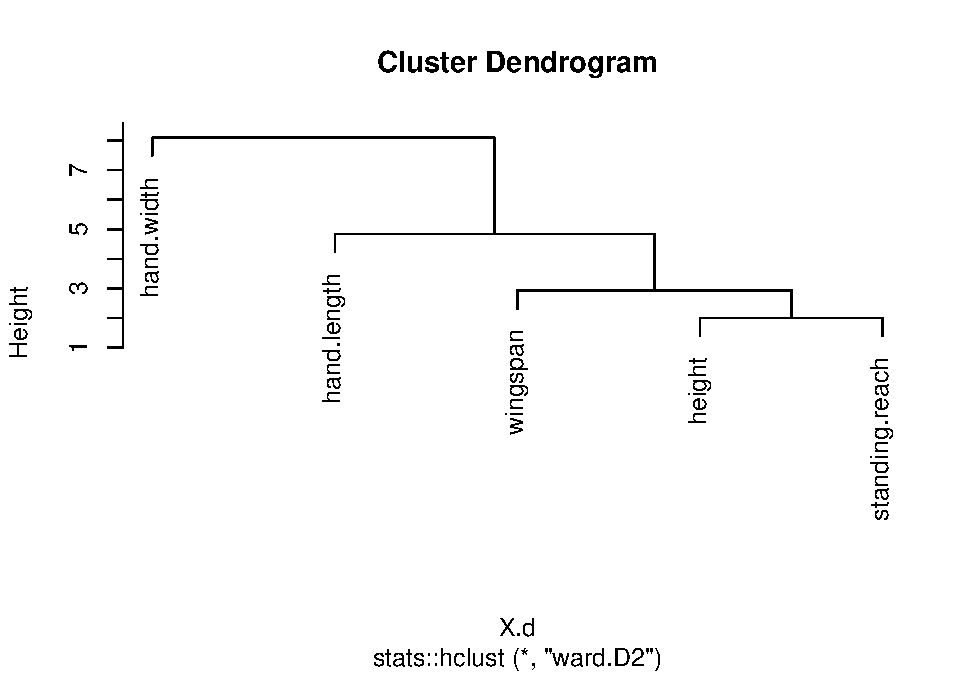
\includegraphics{project-measure-writeup_files/figure-latex/hclust-nba-1.pdf}
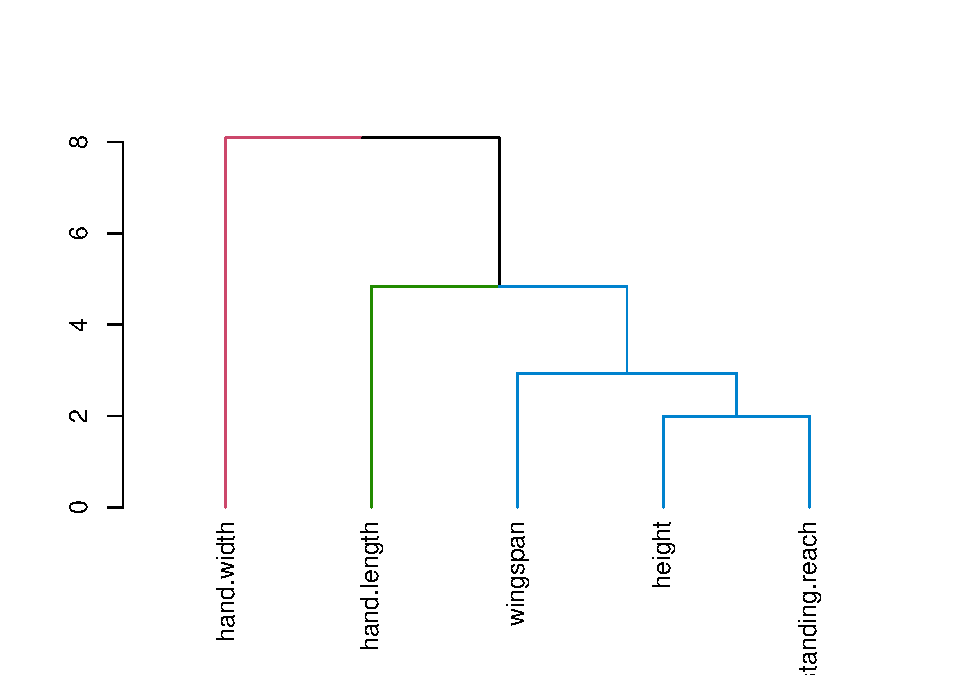
\includegraphics{project-measure-writeup_files/figure-latex/hclust-nba-2.pdf}

\begin{verbatim}
## [1] "Pruning 1 of 3"
## [1] "Pruning 2 of 3"
## [1] "Pruning 3 of 3"
\end{verbatim}

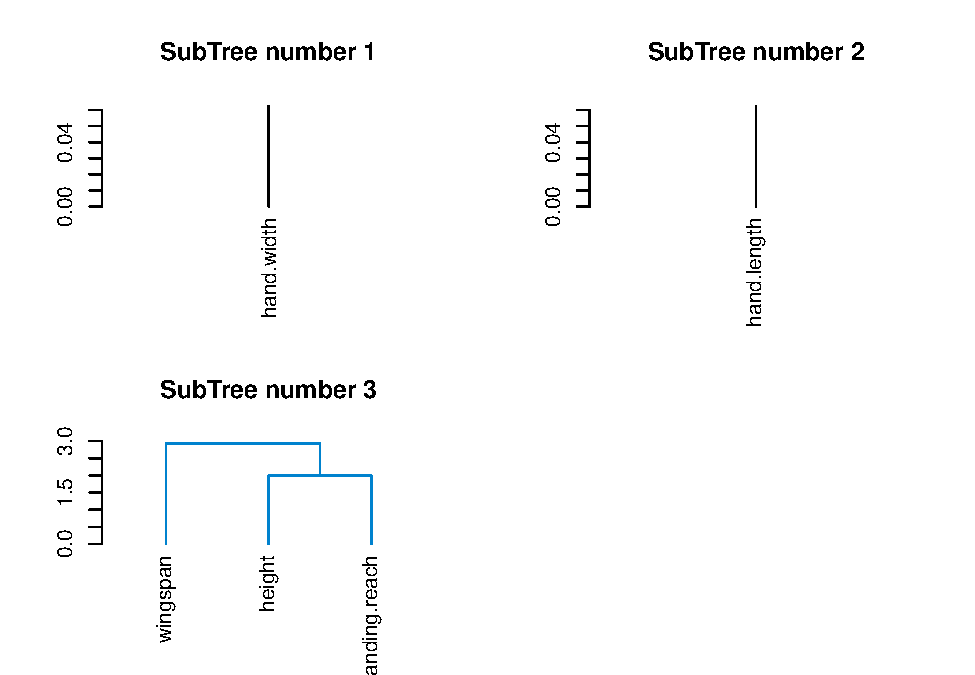
\includegraphics{project-measure-writeup_files/figure-latex/hclust-nba-3.pdf}

\begin{Shaded}
\begin{Highlighting}[]
\KeywordTok{source\_url}\NormalTok{( }\KeywordTok{paste0}\NormalTok{(path.humanVerseWSU,}\StringTok{"master/humanVerseWSU/R/functions{-}EDA.R"}\NormalTok{) );}
\end{Highlighting}
\end{Shaded}

\begin{verbatim}
## SHA-1 hash of file is dd72e464241952b23d5b08d2213099eccf7a86f6
\end{verbatim}

\begin{Shaded}
\begin{Highlighting}[]
\NormalTok{Xs =}\StringTok{ }\KeywordTok{scale}\NormalTok{(measure.df[,}\KeywordTok{c}\NormalTok{(}\DecValTok{1}\NormalTok{,}\DecValTok{2}\NormalTok{,}\DecValTok{3}\NormalTok{,}\DecValTok{4}\NormalTok{,}\DecValTok{5}\NormalTok{)])}
\NormalTok{Xs =}\StringTok{ }\KeywordTok{transposeMatrix}\NormalTok{(Xs)}
\NormalTok{do.nothing =}\StringTok{ }\KeywordTok{perform.hclust}\NormalTok{(Xs,}\DecValTok{3}\NormalTok{) }
\end{Highlighting}
\end{Shaded}

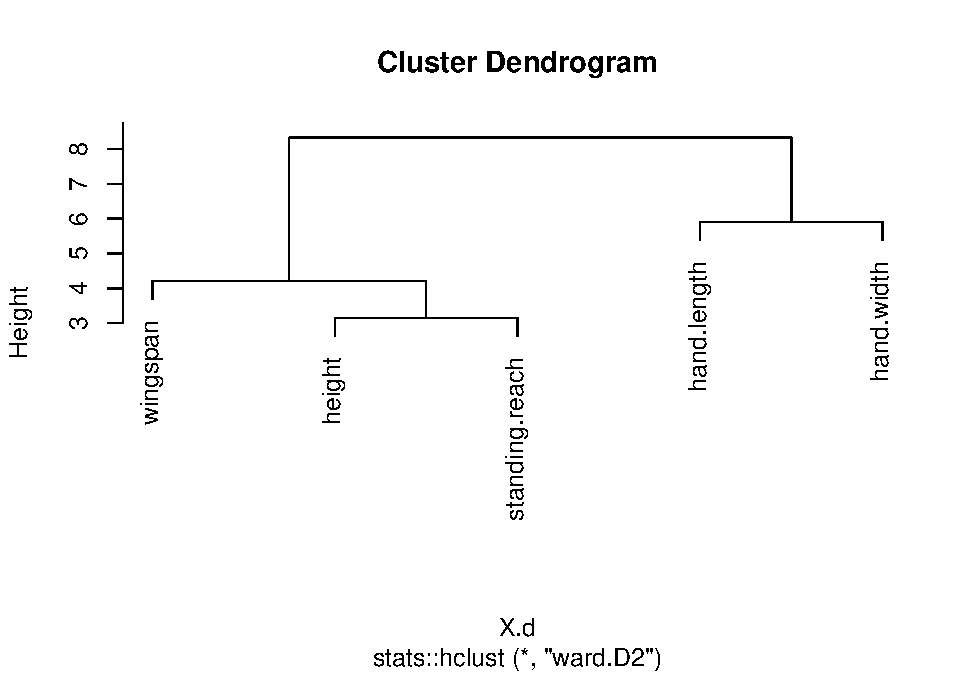
\includegraphics{project-measure-writeup_files/figure-latex/hclust-measure-1.pdf}
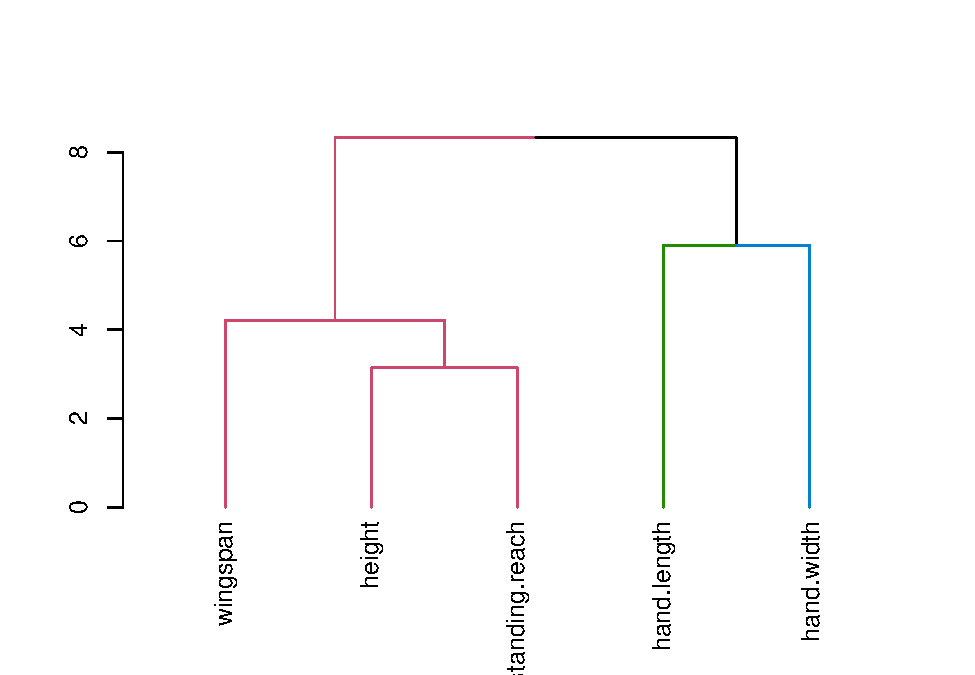
\includegraphics{project-measure-writeup_files/figure-latex/hclust-measure-2.pdf}

\begin{verbatim}
## [1] "Pruning 1 of 3"
## [1] "Pruning 2 of 3"
## [1] "Pruning 3 of 3"
\end{verbatim}

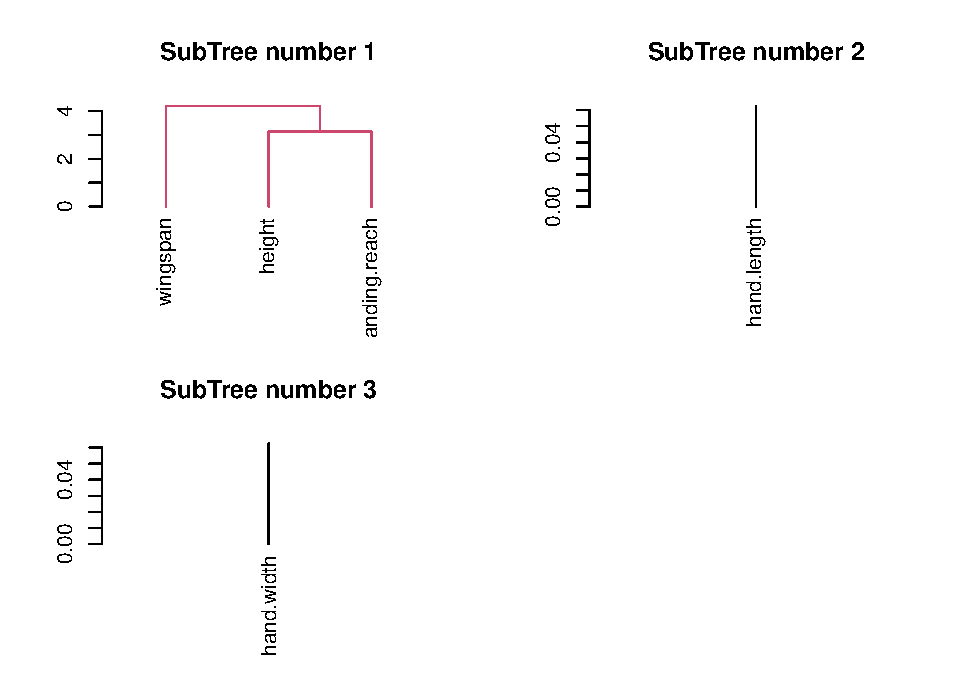
\includegraphics{project-measure-writeup_files/figure-latex/hclust-measure-3.pdf}




%% appendices go here!


\newpage
\theendnotes

%%%%%%%%%%%%%%%%%%%%%%%%%%%%%%%%%%%  biblio %%%%%%%%
\newpage
\begin{auxmulticols}{2}
\singlespacing 
\bibliography{./../biblio/master.bib}

%%%%%%%%%%%%%%%%%%%%%%%%%%%%%%%%%%%  biblio %%%%%%%%
\end{auxmulticols}

\newpage
{
\hypersetup{linkcolor=black}
\setcounter{tocdepth}{3}
\tableofcontents
}



\end{document}